%-----------------------------------------------%
%---------------------------------------------%
%
% BACHELOR OF SCIENCE THESIS
%
% Emanuele Ballarin <emanuele@ballarin.cc>
%
% Prof. Luca Bortolussi, Prof. Fabio Benatti
%
%---------------------------------------------%
%
% Bachelor's Degree in Physics
%
% Dept. of Physics
% University of Trieste, Italy
%
% 24-27/04/2020
%
% A.Y. 2018/2019
%
%
% Authored on 16/04/2020
%
%
%---------------------------------------------%
%-----------------------------------------------%


% Document configuration %
%---------------------------------------------%
\documentclass[a4paper, twoside]{article}
%---------------------------------------------%

% Used packages and configuration %
%------------------------------------------------------------------------%
%\usepackage{fontspec}
%\usepackage{microtype}
\usepackage[utf8]{inputenc}
\usepackage[italian]{babel}
\usepackage{natbib}
\usepackage{graphicx}
\usepackage{amsmath}
\usepackage{mathtools}
\usepackage{wrapfig}
\usepackage{amsfonts}
\usepackage{csquotes}
\usepackage{epigraph}
\usepackage{float}
\usepackage{graphicx,wrapfig,lipsum}
\usepackage{blindtext}
\usepackage{multirow}
\usepackage[ruled,vlined]{algorithm2e}
\usepackage{wrapfig}
\usepackage{graphicx}
\usepackage{babel}
\input{insbox}
\usepackage[font=small,font=it]{caption}

% MARGINS %
\usepackage{geometry}\geometry{top=2.5cm,bottom=2.5cm,left=3cm,right=3cm} % Symmetric
%\geometry{top=2cm,bottom=2cm,right=3cm,left=1.8cm,headheight=15pt}   % Asymmetric

\usepackage{fancyhdr}
\usepackage{bm}
\usepackage{xcolor}
\usepackage[titletoc]{appendix}
\usepackage{upgreek}

% FANCYHDR CONFIG %
\pagestyle{fancy}
\fancyhead{}
\renewcommand{\headrulewidth}{0.4pt}
\renewcommand{\footrulewidth}{0.4pt}
\setcounter{secnumdepth}{4}

% CHAPTER TITLES CONFIG %
\usepackage{titlesec}
\titleformat{\chapter}[display]{\normalfont\Huge\bfseries}{\chaptertitlename\ \thechapter}{15pt}{\Huge}
\titlespacing*{\chapter}{0pt}{-3\baselineskip}{20pt}[3.7cm]% Moves the chapter title out of the text block. Do you really want this?
\assignpagestyle{\chapter}{empty}

\usepackage{nomentbl}
\usepackage{enumitem,calc}
\usepackage{lscape}
\usepackage{setspace}\linespread{1.4}
\usepackage{parskip}
%------------------------------------------------------------------------%


% Document declaration %
%------------------------------------------------------------------------%
\begin{document}
\begin{titlepage}
\newcommand{\HRule}{\rule{\linewidth}{0.5mm}} % Defines a new command for the horizontal lines, change thickness here
\center % Center everything on the page (why unrecognized??)
%------------------------------------------------------------------------%


% HEADINGS %
%------------------------------------------------------------------------%
\vspace{-16mm}
\vspace*{16mm}
\textsc{\LARGE{Università degli Studi di Trieste}}\\[1.5cm] % Name of your university/college
%------------------------------------------------------------------------%


% LOGO %
%------------------------------------------------------------------------%

\includegraphics[width=0.30\linewidth]{logouniv.png} % Include a department/university logo - this will require the graphicx package
%------------------------------------------------------------------------%


% TITLES %
%------------------------------------------------------------------------%
\HRule \\[0.4cm]
{ \huge \bfseries Modelli generativi di modelli neurali artificiali robusti}\\[0.4cm] % Title of your document
{ \LARGE Uno studio preliminare di fattibilità}\\[0.4cm]
\HRule \\[1.5cm]
%------------------------------------------------------------------------%


% AUTHOR %
%------------------------------------------------------------------------%
\begin{minipage}{0.4\textwidth}
\begin{flushleft}
\Large \emph{{Autore:}}\\
{Emanuele} \textsc{{Ballarin}} % Your name
\end{flushleft}
\end{minipage}
~
\begin{minipage}{0.4\textwidth}
\begin{flushleft}
\Large \emph{{Relatore:}} \\
{Prof. Luca}  \textsc{{Bortolussi}} \\ % Supervisor's Name

\emph{{\\ Co-Relatore:}} \\
{Prof. Fabio}  \textsc{{Benatti}}
\end{flushleft}
\end{minipage}\\[2cm]
%------------------------------------------------------------------------%


% DATE and PLACE %
%------------------------------------------------------------------------%
\Large
\textsc{Dipartimento di Fisica\\
A.A. 2018/2019}
\vfill % Fill the rest of the page with whitespace
\end{titlepage}
%------------------------------------------------------------------------%


% LEADING EMPTY PAGE and T.O.C. %
%------------------------------------------------------------------------%
\newcommand{\blankpage}{
	\newpage
	\thispagestyle{empty}
	\mbox{}
	\newpage}

\blankpage
\newpage
\renewcommand{\contentsname}{Indice}  % Easy language compatibility (no additional package)
\setcounter{section}{-1}			  % Index section starts from 0
\tableofcontents  % Uncomment
%------------------------------------------------------------------------%


% ABSTRACT %
%------------------------------------------------------------------------%
\newpage
\section{Abstract}

Il presente lavoro di tesi, redatto in osservanza dei requisiti per il conferimento del titolo di \textit{Laurea in Fisica} (triennale), si occupa di formulare, esplorare e valutare preliminarmente un nuovo approccio originale per il \textit{training} di modelli basati su reti neurali profonde (\textit{Deep Learning}), che siano in grado di soddisfare opportune proprietà di \textit{adversarial robustness} -- ovvero di resistenza a perturbazioni degli input, costruite ad arte con il fine di produrre un comportamento non corretto (o non previsto) nei modelli suddetti -- senza sacrificare la loro accuratezza, o facendolo al più in modo controllabile.

In particolare, l'approccio proposto mira a raggiungere suddetti obiettivi attraverso la generazione dei \textit{pesi} della rete neurale in analisi tramite un modello generativo e un \textit{value network} ausiliario che ne determini la \textit{funzione costo}, entrambi a loro volta reti neurali profonde. Questa modalità di procedere si distingue, da quella attualmente più seguita per il medesimo scopo (e con risultati sicuramente lontani dall'essere definitivi), nel non ricorrere alla \textit{backpropagation} direttamente sul modello in analisi come strategia per produrre \textit{robustezza}.

Dopo aver contestualizzato il paradigma contemporaneo del \textit{Deep Learning} all'interno dei più generali ambiti dell'\textit{Intelligenza Artificiale} e del \textit{Machine Learning} (in particolare quello \textit{statistico} e \textit{probabilistico}), il presente elaborato fornisce un'introduzione ai suoi elementi caratterizzanti e fondativi, ad alcune tecniche collegate -- in uso nel seguito --, e al problema dell'\textit{adversarial robustness} per i modelli così prodotti, insieme ad alcuni esempi di \textit{attacchi} e \textit{difese} già noti.\\
Successivamente, sono proposte una misura di \textit{adversarial robustness globale} e una \textit{performance metric} che tenga esplicitamente conto di un eventuale \textit{tradeoff} tra accuratezza e \textit{robustezza}. Dunque, facendone uso, è dettagliato l'approccio originale proposto e sono altresì descritte le procedure sperimentali che si sono seguite al fine di verificarne preliminarmente il buon comportamento.

Da ultimo, sono riportate le conclusioni maturate grazie a tale esperienza, gli aspetti di maggior validità e di eventuale criticità dell'approccio proposto, e le prospettive di ricerca futura che da esso vengono offerte e suggerite.



% INTRODUCTION %
%------------------------------------------------------------------------%
\newpage
\section{Introduzione}

Sin dalle sue origini, e in misura ben più marcata a partire dalla \textit{Prima Rivoluzione Industriale}, lo sviluppo della civiltà umana è stato caratterizzato dalla realizzazione di strumenti -- di crescente efficacia, efficienza e varietà d'applicazioni -- che potessero migliorare la condizione dei suoi membri e massimizzare la capacità di soddisfacimento dei più disparati bisogni.

Tuttavia, pur in seguito all'avvento delle tecnologie informatiche di massa e sicuramente fino agli anni 10 del secolo in corso, tale tentativo in contesto \textit{di produzione} non si è mai concretizzato nell'automazione di funzioni cognitive di ordine superiore -- quand'anche animali, se non umane -- come il \textit{ragionamento deduttivo}, l'\textit{inferenza induttiva e causale}, l'\textit{elaborazione delle informazioni sensoriali} (\textit{visione} prima fra tutte), la \textit{capacità decisionale}.

Il tentativo di affrontare in modo rigoroso e quantitativo il problema del \textit{funzionamento della mente}, dell'apprendimento e della cognizione -- con il fine derivarne un modello ed, eventualmente, simularlo artificialmente -- può essere però già trovato nei lavori di McCulloch \& Pitts (1943), Hebb (1949), Minsky \& Papert (1969) e Hopfield (1980).\\
In particolare, tali approcci si distinguono dal pur popolare (all'epoca come oggi) filone della \textit{logica} (anche computazionale) e dei sistemi di deduzione automatica -- con finalità parzialmente sovrapposte -- per il loro carattere estremamente generale, non orientato alla specifica attività da svolgere, e fondato essenzialmente sulla formalizzazione e modellazione matematica del funzionamento dei neuroni e delle loro interconnessioni, in forma approssimata ed essenziale.

Tale dicotomia metodologica (non priva tuttavia di reciproche influenze e commistioni) ha portato tradizionalmente a suddividere il vastissimo ambito di ricerca della cosiddetta \textit{Intelligenza Artificiale} nel filone \textit{simbolico} (il secondo, orientato principalmente alla manipolazione di simboli e predicati con finalità deduttive) e quello \textit{connessionista} (il primo, ispirato al funzionamento degli aggregati di neuroni biologici \textit{lato sensu}, e oggi talvolta citato, senza una chiara convenzione sull'uso dei termini, anche con i nomi di \textit{cognitive computing} o \textit{neuroscienze matematiche/computazionali}).

Per ciascuno di questi due approcci alla ricerca \textit{fondamentale}, nel corso degli ultimi cinquant'anni, sono state sempre più spesso proposte eventuali applicazioni industriali e commerciali, con una discreta dominanza del filone \textit{simbolico} negli anni '80 e '90, per poi assistere a una ripresa di popolarità del \textit{connessionismo} culminata (o meglio, culminante tutt'oggi) nella \textit{Deep Learning revolution} iniziata durante lo scorso decennio.

L'influente e più che ventennale lavoro dei gruppi di ricerca guidati da Hinton, LeCun e Bengio -- proprio per questo insigniti dell'\textit{ACM Turing Prize} nel 2018 --, l'accesso a sempre più potenti e meno costosi calcolatori equipaggiati con \textit{hardware} di consumo adatto ai calcoli richiesti da questo particolare approccio (come le \textit{GPU} parte delle schede grafiche dedicate) e il crescente coinvolgimento e finanziamento in tale direzione da parte di soggetti privati, interessati alle applicazioni commerciali del paradigma, sono considerati i fattori di maggiore rilevanza per spiegare tale popolarità senza precedenti. La necessità di una notevole quantità di dati per garantire il corretto \textit{training} dei modelli neurali profondi -- congiunta a un periodo come quello attuale in cui connettività a Internet diffusa, dispositivi \textit{smart} per uso personale e il cosiddetto \textit{Internet of Things} possono proprio contribuire alla loro facile raccolta -- spiega infine le ragioni del successo commerciale di questa tecnologia.

All'attuale \textit{stato dell'arte}, il \textit{Deep Learning} si dimostra il più \textit{capace} ed \textit{espressivo} \textit{framework} noto di \textit{modellazione statistico-probabilistica}, capace di successi talvolta conosciuti anche dal grande pubblico. Da segmentazione e riconoscimento d'immagini (e pure facciale), al riconoscimento vocale, alla classificazione, traduzione e addirittura scrittura \textit{ex-novo} di testi, documenti e \textit{corpora} letterari multi-linguistici, alla generazione di audio, video e immagini realistici e originali. Ma pure -- con un carattere maggiormente applicativo -- alla diagnosi clinica \textit{computer-aided} quando non completamente automatica, alla guida autonoma di autoveicoli in ambiente controllato, e a un'automazione industriale dotata di un'\textit{intelligenza} più simile a quella umana.

Dalla precedente elencazione -- pur estremamente ridotta e sicuramente non esaustiva -- dei più significativi \textit{successi} (anche se, più correttamente, si dovrebbe semplicemente parlare di casi in cui si è riusciti ad ottenere il comportamento desiderato) del paradigma si potrebbe essere colti dalla facile impressione che il \textit{Deep Learning} sia uno strumento \textit{definitivo}, completamente conosciuto, controllabile nelle sue caratteristiche, e bisognoso solo di miglioramenti incrementali e nuove applicazioni in cui eccellere.

La realtà, tuttavia, è meno rosea. Sebbene il paradigma sia ragionevolmente maturo, esplorato, e capace di raggiungere obiettivi mai stati alla portata della modellazione statistica tradizionale, esso può soffrire di alcune debolezze. Queste possono essere genericamente raccolte in tre gruppi principali: la \textit{fame di risorse} (dati e potenza di calcolo) necessaria al suo corretto funzionamento, la scarsa o assente \textit{interpretabilità} dei modelli così prodotti e la scarsa \textit{robustezza ad adversarial perturbations}.

Il presente lavoro si concentrerà sull'ultima classe di debolezze -- forse tra tutte quella che maggiormente ostacola l'adozione del \textit{Deep Learning} in ambiti in cui un errore, indotto casualmente o anche di proposito, può comportare rischi incontrollabili o danni ingenti. È infatti generalmente possibile, data una rete neurale profonda in grado di assolvere correttamente alla sua funzione prevista, produrre opportunamente input tali da provocare in essa un comportamento scorretto, imprevisto, o addirittura arbitrariamente controllabile.

Per raggiungere il nostro scopo, e dunque indagare preliminarmente la ragionevolezza di un nuovo approccio atto a contenere il problema, forniremo nel seguito anche un'introduzione generale a taluni aspetti di \textit{Machine Learning} e \textit{Deep Learning}, e al problema dell'\textit{adversarial robustness}.
%------------------------------------------------------------------------%



% ML PRIMER %
%------------------------------------------------------------------------%
\newpage
\section{Cenni di \textit{Statistical Machine Learning}}

In virtù del suo carattere generale, amplissimo e fortemente interdisciplinare, il tema dell'\textit{Intelligenza Artificiale} può essere affrontato da numerosi punti di vista, a differenti livelli di formalizzazione e misurabilità.

L'approccio da cui ha avuto origine il \textit{Deep Learning}, e che seguiremo, muove dall'assunto secondo cui l'attività cognitiva possa essere modellata formalmente in linguaggio matematico -- anche facendo ricorso agli strumenti della statistica e del calcolo delle probabilità --, riducendola così a computazione algoritmica, ancorché arbitrariamente ricca ed elaborata. Tale idea (il \textit{computazionalismo cognitivo}), purificata (almeno in questa sede) da ogni possibile pretesa di verità sul mondo biologico, rappresenta il contesto primario in cui s'inseriscono i tentativi contemporanei di riprodurre -- quantomeno nei loro effetti -- le funzioni cognitive superiori animali, e costituisce forse l'unica base adeguata per eventuali applicazioni ingegneristiche che vogliano sfruttarne le potenzialità.\\
Questa ancora estesissima macro-area viene talvolta menzionata con il nome di \textit{Intelligenza Computazionale (Artificiale)}.

Restringendo ulteriormente il campo, ci concentreremo in particolare sul \textit{Machine Learning} (di cui il \textit{Deep Learning} è espressione): un approccio rigoroso, quantitativo e orientato all'applicazione (piuttosto che alla finalità conoscitiva). Oggetto di studio di questa disciplina è una particolare classe di algoritmi -- e la loro implementazione al calcolatore -- detti \textit{di apprendimento}, il cui obiettivo consiste nel
\begin{displayquote}
\textit{[...] dotare un sistema computazionale che li esegue della capacità di apprendere dall'esperienza senza essere esplicitamente programmato} \\(Samuel, 1959).
\end{displayquote}


\subsection{Il carattere statistico del \textit{ML}}

La definizione appena riportata, decisamente vaga e incline a essere fraintesa, si può chiarire e formalizzare spiegando che
\begin{displayquote}
	\textit{Un programma informatico impara da un'esperienza $E$ con riferimento ad un'attività $T$ e una misura di prestazioni $P$ se le sue prestazioni misurate da $P$ nello svolgimento dell'attività $T$ migliorano noto $E$.} \\(Mitchell, 1998).
\end{displayquote}

Da ciò, anche senza il bisogno di scendere nei dettagli tecnici riguardo alla natura di $T$, $P$ ed $E$ (quest'ultima generalmente identificabile come una certa quantità di \textit{dati} forniti in input all'algoritmo d'apprendimento), si può cogliere il legame del \textit{Machine Learning} con la statistica come teoria asintotica.

In ultima analisi, un algoritmo d'apprendimento -- in una prima fase detta \textit{di training}, in cui è confrontato con una porzione di dati in ingresso già noti e i corrispettivi output desiderati, o anche semplicemente con una proprietà ben definita degli output attesi  -- deve sviluppare un \textit{modello computazionale} in grado di cogliere l'essenza dell'attività che è chiamato ad apprendere, e in grado di mappare i possibili input (anche non necessariamente incontrati in fase di \textit{training}) nell'output adeguato.\\
Per quanto ci si aspetti che -- considerato un algoritmo d'apprendimento ideale -- le sue prestazioni migliorino arbitrariamente al continuare del \textit{training}, quest'ultimo può essere interrotto in qualunque momento e -- in una seconda fase detta \textit{d'inferenza} -- il modello suddetto può essere utilizzato per processare degli input d'interesse, al meglio di quanto appreso.

In virtù di tale similitudine con la modellazione statistica tradizionalmente intesa, il presente ambito di ricerca prende spesso il nome, più preciso, di \textit{Statistical Machine Learning}.

Qualora, infine, l'input e l'output di suddetti algoritmi siano rappresentati da distribuzioni di probabilità -- o loro funzioni -- si parla di \textit{Machine Learning probabilistico}.


\subsubsection{L'esempio dei modelli regressivi lineari}

Prima di addentrarci ulteriormente nella spiegazione degli aspetti più rilevanti della teoria del \textit{Machine Learning} appunto detto \textit{statistico}, può essere utile tracciare un parallelo tra quanto esposto e la procedura di \textit{fit} di un modello regressivo lineare -- che può essere vista come un semplice algoritmo di \textit{Machine Learning} qualora implementato da un programma informatico.

Supponendo di aver registrato un certo numero $n$ di coppie di dati reali $(x_1, y_1), (x_2, y_2), \dots,(x_n, y_n)$, che si ipotizzano essere legate da una relazione lineare del tipo $y = mx + c$ è possibile stimare dei parametri $\hat{m}, \hat{c}$ tali che $\hat{y_{x'}} = \hat{m}x' + \hat{c}$ costituisca un modello dello specifico fenomeno osservato e consenta di stimare $\hat{y_{x'}}$ associato a qualunque $x'$ prodotto dal medesimo fenomeno in analisi.

Per riuscire in tale intento, è possibile, per esempio, determinare analiticamente i valori di $\hat{m}, \hat{c}$ tali che lo scarto quadratico medio sui dati osservati $MSE = \frac{1}{n}\sum_{i=1}^{n}{(\hat{y_{x_i}} - y_{x_i})^2}$ sia minimo per il modello.

In tale procedimento, che sebbene rappresenti un esempio molto specifico è facilmente generalizzabile a tutti i casi che andremo ad osservare, si può identificare in un \textit{task} $T$ l'attività di prevedere $y$ noto un qualunque $x$, l'esperienza $E$ nell'insieme delle coppie $(x_i, y_i)$, $P$ in $MSE$ e l'algoritmo d'apprendimento in quanto tale nella procedura analitica che consente di calcolare $\hat{m}, \hat{c}$.

L'esempio appena proposto, completo pur nella sua semplicità, sarà talvolta ripreso ed esteso nel seguito con il fine di esemplificare altri significativi concetti propri della teoria del \textit{Machine Learning}.


\subsection{Breve sistematica degli algoritmi di apprendimento}

Nella loro ancor numerosa varietà, gli algoritmi d'apprendimento possono essere suddivisi in diversi modi, in base alle specifiche proprietà e interrelazioni a cui viene data importanza. In seguito, rinunciando a una finalità enciclopedica, forniamo due possibili partizioni, la cui differenza tornerà utile.


\subsubsection{Dal punto di vista probabilistico}

Ponendoci sotto le ipotesi del \textit{Machine Learning probabilistico}, chiamando genericamente con $x$ la variabile aleatoria associata agli input e -- qualora presenti -- con $y$ quella associata agli output, possiamo distinguere

\begin{itemize}
	\item {l'\textbf{apprendimento generativo}, il cui scopo è quello di descrivere l'intera distribuzione di probabilità degli input $p(x)$, o quella congiunta di input e output $p(x,y) = p(x)p(y|x)$, o anche loro funzioni e trasformazioni;}
	\item {l'\textbf{apprendimento discriminativo}, il cui scopo è invece quello di determinare la distribuzione degli output noti gli input $p(y|x)$ o una sua statistica (come il valore di $y$ più probabile, noto $x$).}
\end{itemize}


\subsubsection{Sulla base della quantità di supervisione richiesta}

In maniera più generale, inoltre, possiamo partizionare gli algoritmi d'apprendimento in base all'ammontare di supervisione (inteso nel senso di dati già noti o analizzati) che richiedono per il loro funzionamento. In particolare

\begin{itemize}
	\item {l'\textbf{apprendimento supervisionato} consiste nell'apprendere un modello dei dati -- note alcune coppie di input e output associati -- con il fine di poter applicare il modello risultante a un nuovo input per prevedere l'output corrispondente o la sua distribuzione.\\
	Di questa classe fanno parte la regressione (output continui) e la classificazione (output discreti o categorici) e, nel caso probabilistico, si tratta quasi sempre di apprendimento \textit{discriminativo}.}

	\item {L'\textbf{apprendimento non supervisionato} ha invece l'obiettivo di apprendere proprietà o trasformazioni dei soli dati di input. Questo si può concretizzare nell'abilità di apprenderne un modello generativo, ma anche -- ad esempio -- nel loro \textit{clustering}.}

	\item {L'\textbf{apprendimento per rinforzo}, infine, punta a determinare quale azione -- tra un ventaglio di possibilità -- sia preferibile intraprendere in una determinata situazione, nota soltanto una \textit{funzione di reward} che è associata ad ogni possibile stato e comportamento del sistema. Questo aspetto, meno statisticamente trattabile, ha forti legami con i problemi di \textit{controllo ottimo} e la teoria delle decisioni.}
\end{itemize}

È a tal punto necessario precisare, tuttavia, che nessuna delle suddivisioni proposte rappresenta una compartimentazione rigida di un'area di ricerca varia e in costante evoluzione. Sebbene utili con finalità didascaliche, tali partizionamenti vengono spesso superati nel caso di \textit{tasks} particolari come la generazione condizionale di dati (l'uso -- cioè -- di un modello che abbia appreso la distribuzione di probabilità $p(x|y)$) o in alcuni sistemi di \textit{Machine Learning} più avanzati dove diverse parti -- ciascuna imparando un modello specifico e con differenti caratteristiche -- collaborano al raggiungimento di un particolare obiettivo comune d'interesse.


\subsection{Assunzione distribuzionale, \textit{loss function} e generalizzazione}

Come già menzionato in precedenza, l'aspetto che forse più fra tutti contribuisce alla notevole popolarità degli approcci di \textit{Machine Learning} è la possibilità che questi offrono di approcciare problemi definiti solo implicitamente, o attraverso la semplice presentazione di esempi (sotto forma di dati in fase di \textit{training}) costituiti da coppie di \textit{input-output} considerati corretti.

L'efficacia di un simile approccio, tuttavia, non può che dipendere dalla possibilità -- una volta terminato il training -- di applicare il modello così prodotto su dati (o per generare dati, nel caso, ad esempio, di un modello generativo) differenti da quelli già sfruttati.\\
Per tornare all'esempio del modello regressivo lineare, una volta determinati dai dati di \textit{training} i parametri $\hat{m}, \hat{c}$, l'espressione $\hat{m}x + \hat{c}$ può essere calcolata per qualunque valore di $x$ reale per ottenere una stima della $y$ corrispondente.

\subsubsection{L'assunzione distribuzionale}

Affinché questo sia possibile, innanzitutto, è necessario che siano rispettate alcune condizioni preliminari sui dati di \textit{training} utilizzati, tali da garantire il rispetto della cosiddetta \textit{assunzione distribuzionale}, tipica pure di moltissimi metodi statistici più tradizionali.

Una formulazione di questo principio consiste nel garantire che i dati forniti all'algoritmo d'apprendimento in fase di \textit{training} siano statisticamente rappresentativi del fenomeno che si intende indagare: assumendo che tutti i possibili dati prodotti dal fenomeno seguano una certa distribuzione di probabilità, il processo con cui gli esempi di \textit{training} vengono scelti deve essere tale da preservare tale distribuzione, se iterato un numero arbitrario di volte.

\subsubsection{La \textit{loss function}}
Un secondo elemento a cui è importante prestare attenzione è il criterio con cui un algoritmo d'apprendimento costruisce un modello dei dati. L'unica misura in grado di quantificare la bontà di tale modello è la già menzionata \textit{misura delle prestazioni} dell'algoritmo $P$.

In generale, dato un certo modello $F_{\boldsymbol{w}}$ dipendente da un vettore $\boldsymbol{w}$ di parametri che devono essere appresi, e un insieme di esempi di \textit{training} $\mathcal{T} = \left\{ t_1, \dots, t_n \right\}$, è possibile introdurre una \textit{misura delle prestazioni} $\mathbb{L}$ genericamente funzione di $\boldsymbol{w}$ (o dell'intero modello in quanto tale $F_{\boldsymbol{w}}$) e degli elementi di $\mathcal{T}$ tale che essa sia minima (o massima) in corrispondenza dei particolari parametri $\boldsymbol{\hat{w}}$ che producono il modello reputato migliore.

Nel contesto della stima di parametri (e conseguente costruzione di modelli che fanno uso di tali stime), il \textit{likelihood} $\mathcal{L} = P\left(\left\{ t_1, \dots, t_n \right\}|\boldsymbol{w}\right)$ (o, se si desidera una \textit{funzione costo} vera e propria, il suo opposto $-\mathcal{L}$) è una comune misura di prestazioni per il modello appreso, consistente nella probabilità di osservare i dati di training, noto il vettore dei parametri di un modello che li genera.

Altre \textit{losses} sono tuttavia possibili, a patto di conoscerne l'andamento in corrispondenza dei parametri che si reputano produrre il modello migliore -- e ricordando che il suo valore rappresenta l'unica informazione di \textit{feedback} all'algoritmo d'apprendimento riguardo al modello che sta producendo.

\subsubsection{Il problema della generalizzazione}

A questo punto della trattazione, una domanda potrebbe sorgere spontanea: anche ammettendo che l'assunzione distribuzionale sia rispettata, ma sapendo che in generale l'ammontare di dati disponibili per il \textit{training} è limitato, com'è possibile essere sicuri che l'algoritmo d'apprendimento utilizzato apprenda un modello del fenomeno in esame e non a copiare gli esempi \textit{verbatim}?

La domanda non è ininfluente. Tornando ancora una volta all'esempio della regressione lineare, immaginiamo un ipotetico algoritmo d'apprendimento che sia in grado semplicemente di associare a ciascun valore $x_i$ al suo $y_i$ corrispondente nelle varie coppie $(x_i, y_i)$ fornite in fase di \textit{training}.\\
Un simile algoritmo, per quanto il modello prodotto non sia nemmeno applicabile per valori di $x$ esterni al \textit{training set} produrrebbe un valore di $MSE$ sicuramente minore rispetto a qualunque modello lineare per punti non perfettamente allineati.

Il problema di come garantire che venga \textit{appreso un modello dei dati, senza apprendere semplicemente i dati stessi} prende il nome di \textit{problema della generalizzazione} e non è risolubile in forma generale.

Un ulteriore approfondimento di questa e alcune tematiche collegate, tuttavia, porta a definire una serie di aspetti a cui prestare particolare attenzione nel tentativo di sviluppare e utilizzare algoritmi d'apprendimento capaci di una buona generalizzazione.

A ciò saranno dedicati i paragrafi che seguono.


\subsection{La \textit{model selection}}

Per introdurre l'argomento che andremo a trattare, può essere significativo considerare una domanda in apertura. Supponendo di avere due modelli -- fissati -- che siano stati allenati sul medesimo \textit{training set} (facendo sempre riferimento al caso regressivo: le coppie di coordinate $(x_i, y_i)$) e attraverso la medesima scelta per la \textit{loss function} (che, per esempio, si può supporre funzione solo dei dati di \textit{training} e degli output del modello), in cosa saranno diversi tali modelli? Quale dei due sarà opportuno preferire per meglio risolvere il problema in esame, in relazione alle sue prestazioni, ma anche alla sua capacità di generalizzazione?

È scontato che la questione possa facilmente essere estesa anche a più di due modelli, e che -- specialmente se il \textit{training} è una procedura dispendiosa di tempo o risorse -- una decisione in tal senso possa dover essere presa prima ancora d'iniziarlo o di poter confrontare i due modelli appresi su di un problema di test pensato allo scopo.

Il problema della \textit{model selection}, tipico anche degli approcci statistici tradizionali, può essere meglio formalizzato andando a considerare il significato profondo associato alla costruzione di un modello -- anche se, come si vedrà meglio in seguito, le risposte seguite dalla statistica tradizionale e dal \textit{Machine Learning} (in particolare quello \textit{deep}) per affrontarlo seguono strade diverse.

\subsubsection{Il \textit{Data coding}}

Immaginiamo dunque di essere interessati a un particolare fenomeno, e cioè a determinate proprietà di uno o più eventi che siamo in grado di osservare -- anche solo in parte.

Per poter procedere alla sua modellazione matematica è innanzitutto necessario definire con precisione una \textit{codifica} per suddette proprietà d'interesse: in altre parole occorre stabilire una convenzione con cui rappresentare il contenuto delle osservazioni e i risultati che dal modello vogliamo ricavare. Nell'ambito delle scienze naturali, solitamente, questo coincide con i risultati numerici di operazioni di misurazione meticolosamente definite -- che pur però non rappresentano l'unica scelta possibile in generale.

Nel caso di un modello per la classificazione d'immagini digitali -- ad esempio -- l'input potrebbe essere codificato come la matrice riportante, pixel per pixel in un ordine prestabilito, le coordinate corrispondenti al colore di tale pixel in uno spazio cromatico discreto opportuno. Nel caso di un segnale audio, si potrebbe trattare della sua forma d'onda campionata a frequenza prestabilita e così via. Analogamente: in caso di un output atteso a carattere numerico si può scegliere direttamente tale valore; nel caso di un problema di classificazione, invece, l'output può essere descritto come un vettore avente dimensione il numero delle classi e, per ciascuna di esse, recante la probabilità con cui l'input vi appartiene.

Nella loro varietà, tuttavia, un aspetto cruciale va tenuto in considerazione -- specialmente per quanto riguarda il \textit{coding} dei dati forniti in fase di \textit{training} --: per quanto adeguato e potente il modello, questo non sarà mai in grado di cogliere aspetti del fenomeno che non siano rappresentabili (direttamente o indirettamente) attraverso la codifica scelta.

Per questa ragione -- specie avendo a disposizione una adeguata potenza di calcolo per processare importanti moli di dati in un tempo non ritenuto eccessivo --, si preferiscono in generale codifiche il più possibile generali e tali da preservare l'intero contenuto informativo del fenomeno osservato. È eventualmente delegato all'algoritmo d'apprendimento e al modello da esso prodotto il compito di selezionare gli aspetti rilevanti dai dati forniti e codificati.

\subsubsection{Pesi, architetture, iperparametri}

In secondo luogo, la possibilità di apprendere un modello dai dati -- e, in generale, di utilizzare modelli per la descrizione di un fenomeno -- è legata ad un'altra assunzione. Quella secondo cui le osservazioni riguardo al fenomeno in esame (opportunamente codificate, ed eventualmente soggette a rumore anche statistico) siano espressione di un processo -- potenzialmente stocastico -- che, sebbene in generale intrattabile e incognito al modellista, possa essere colto da un processo più semplice, trattabile e descrivibile in linguaggio matematico e probabilistico. Questo \textit{processo più semplice} altro non è che il modello appreso, utilizzato in fase \textit{d'inferenza}.

Nel momento in cui un algoritmo d'apprendimento costruisce un modello dei dati che gli vengono forniti, questo si traduce quasi sempre nella determinazione di quei parametri -- detti \textit{pesi} e indicati solitamente con il vettore $\boldsymbol{w}$ in corrispondenza dei quali il modello così prodotto minimizza una \textit{loss} $\mathbb{L}$.

Questi, tuttavia, non sono l'unica variabile in gioco per la determinazione della bontà e della capacità di generalizzazione del modello stesso.

Innanzitutto, fissati prima ancora dell'inizio del \textit{training} sono la famiglia a cui il modello appartiene -- detta più propriamente la sua \textit{architettura}, tenendo conto anche di modelli compositi come quelli gerarchici -- e l'algoritmo di training in quanto tale, cioè la procedura che deve essere eseguita dal calcolatore per determinare dai dati il vettore $\boldsymbol{\hat{w}}$ che meglio stima $\boldsymbol{w}$, noti la famiglia del modello e i dati di \textit{training}.

Questi aspetti, a loro volta, possono dipendere da variabili che ne determinano le caratteristiche e che non è possibile o non si vuole apprendere. Tali variabili sono dette \textit{iperparametri} del modello (o dell'algoritmo di \textit{training}) -- a titolo di esempio non esaustivo: il grado di un modello regressivo polinomiale, dei coefficienti che compaiono nella \textit{loss}, il numero di \textit{clusters} in cui partizionare i dati.

Propriamente definita, quindi, la già citata \textit{model selection} è l'insieme delle tecniche e procedure che portano a selezionare architettura e iperparametri di un modello.

Concludiamo la presente sezione ricordando un risultato rilevante in relazione al contesto e che -- nonostante ad una prima enunciazione possa sembrare significativo del contrario -- conferma l'importanza della selezione dei modelli e degli algoritmi di \textit{training} più adatti allo scopo che si sta cercando di raggiungere.

Una conseguenza del \textit{No free-lunch Theorem per il Machine Learning} (Wolpert, 1996) è appunto il fatto che

\begin{displayquote}
	\textit{Dato un certo numero di algoritmi d'apprendimento -- o d'inferenza statistica -- e una metrica che ne misuri le prestazioni, questi risultano essere equivalenti rispetto a tale metrica mediata su tutti i possibili problemi d'apprendimento che possono essere concepiti.} \\(Wolpert, 2005).
\end{displayquote}

Ciò, oltre a evidenziare l'impossibilità a formulare un unico algoritmo d'apprendimento che, organicamente, sia in grado di risolvere tutti i problemi che è capace di affrontare, dimostra altresì l'importanza di scegliere accuratamente architettura e iperparametri dei modelli, se si vuole trarre vantaggio dal loro uso.


\subsubsection{Espressività e capacità dei modelli}

In generale, non esistono tecniche universali che consentano di determinare a priori -- posto un problema e forniti dei dati -- quale algoritmo d'apprendimento, architettura del modello appreso o iperparametri produrranno i migliori risultati per il problema in esame. Sicuramente utile allo scopo, può essere il confronto diretto tra distinti modelli, una volta allenati, su un problema di soluzione nota che sia rappresentativo del contesto in cui il modello dovrà essere utilizzato (la \textit{validazione} del modello).

La possibilità di testare -- tuttavia -- tutti i modelli \textit{concepibili} che si possano prestare alla risoluzione di un \textit{task} è impraticabile e, in generale, va ristretta quando necessario a un campo assai limitato, vista la generale dispendiosità associata al \textit{training} di un modello.

È qui utile ricordare, prima di procedere con l'analisi di alcuni aspetti in grado di guidare potenzialmente il processo di \textit{model selection} preliminare, che qualunque operazione atta a restringere la ricerca dei modelli a architetture o iperparametri particolari -- non dettata dell'uso di una \textit{performance metric} -- è espressione di una scelta, di un tentativo o di una proprietà riguardo al fenomeno modellato, che viene imposta \textit{by design} sul modello appreso.

Per procedere, ricordiamo l'esempio introdotto inizialmente: l'esigenza di modellare la dipendenza tra due dati numerici reali $x$ e $y$ di cui sono note le coppie $\mathcal{T} = \left\{(x_1, y_1), (x_2, y_2), \dots,(x_n, y_n) \right\}$ per un certo $n$ finito. Come di consueto, tale esempio specifico potrà essere facilmente generalizzato a tutte le diverse tipologie d'algoritmi precedentemente descritte.

La prima scelta che occorre effettuare ha a che fare con la famiglia a cui il modello appartiene, ovverosia con la sua \textit{espressività}. Questa proprietà descrive la varietà di caratteristiche (delle frontiere decisionali nel caso di un classificatore, della distribuzione degli output per un modello generativo, etc...).

A titolo di esempio, i punti identificati dalle coppie in $\mathcal{T}$ potrebbero essere descritti con una funzione polinomiale, oppure con una spezzata poligonale, o ancora con una funzione trigonometrica. A tale proposito, a meno che non sussistano ragioni \textit{di principio} che facciano propendere per una scelta particolare, si preferiscono in accordo con il principio del \textit{rasoio di Occam} funzioni elementari, la cui espressività sia eventualmente controllabile attraverso un iperparametro: è questo il caso -- ad esempio -- del grado di un polinomio.

Nel momento in cui da un iperparametro di questo tipo dipenda il numero di pesi che sarà necessario apprendere per un certo modello (ancora una volta proprio analogamente al grado di un polinomio, a cui è associato il numero di coefficienti moltiplicativi dei vari termini), si parlerà di esso come di un \textit{indice di capacità}.

Mentre lo \textit{hyperparameter tuning} in generale è un aspetto spesso basato sulla ricerca sperimentale dei valori migliori -- eventualmente assistita da ricerca casuale, euristiche o tecniche di meta-ottimizzazione come l'\textit{ottimizzazione Bayesiana}, la scelta della \textit{capacità} di un modello è un ambito molto più studiato e \textit{principled}.

\subsubsection{Parametrizzazione dei modelli: \textit{underfitting} e \textit{overfitting}}

A tal proposito, proviamo a riflettere sulle ricadute della scelta della \textit{capacità} di un modello, partendo dal presupposto di conoscere la natura del processo stocastico che produce i dati a cui siamo interessati.

Come al solito, useremo l'esempio della regressione bidimensionale senza con questo voler indicare che le riflessioni del seguito siano ristrette a tale caso specifico.

Immaginiamo di essere interessati a un fenomeno descritto (esattamente) dalla relazione

$$
Y = f_{\boldsymbol{w}}(X)
$$

in cui $X$, $Y$ sono due variabili aleatorie ed $f_{\boldsymbol{w}}$ una funzione polinomiale nota di ordine $k$ dipendente dal vettore $\boldsymbol{w} \in \mathbb{R}^k$ dei coefficienti moltiplicativi.

A causa del rumore statistico associato al processo di misura, ipotizziamo che venga introdotto un rumore Gaussiano su $Y$, $\epsilon \sim \mathcal{N}(0, \sigma^2)$ cosicché i dati di \textit{training} $\mathcal{T} = \left\{(x_1, y_1), (x_2, y_2), \dots,(x_n, y_n) \right\}$ siano descrivibili come una realizzazione di

$$
y_i = f_{\boldsymbol{w}}(x_i) + \epsilon
$$

Volendo, con il nostro algoritmo d'apprendimento, ottenere un modello per $f_{\boldsymbol{w}}$ -- per scelta polinomiale, che denotiamo con $\mathcal{P}_{d, \boldsymbol{\hat{w}}}$ di grado $d$ e avente coefficienti moltiplicativi le coordinate di $\boldsymbol{\hat{w}} \in \mathbb{R}^d$ -- abbiamo la necessità di determinare il valore ottimale di $d$.

A posteriori, sappiamo che il miglior modello del fenomeno è ottenibile da $d = k$, ma quest'informazione non è nota in fase di \textit{model selection} preliminare.

Ci si prospettano dunque due possibilità, in base alla scelta di $d$:

\begin{itemize}
	\item {Per $d < k$ la capacità del modello è inadatta a cogliere la relazione d'interesse e, per questo, il modello appreso -- per quanto ottimale per quel numero di pesi da apprendere -- non sarà generalmente adeguato allo scopo previsto. Si dice che il modello si trova in \textit{underfitting} rispetto ai dati (o al fenomeno d'interesse), o che è \textit{sottoparametrizzato}.}
	\item {Per $d \geq k$ il modello è teoricamente in grado di cogliere la relazione d'interesse.}
\end{itemize}

Ciò detto, è tuttavia da notare che la capacità teorica a cui si fa riferimento nel secondo punto (anche per assurdo nel caso $d=k$) non garantisce che un modello adeguato venga appreso: a titolo d'esempio i dati di \textit{training} potrebbero essere troppo scarsi (si pensi al caso limite $n=1$), o campionati da una \textit{coda} della distribuzione di $\epsilon$.

Oppure, cosa ben più frequente, una scelta di $d \gg k$ (accade già nel caso $d \geq n$) porta ad ottenere un modello polinomiale che -- nella condizione dei migliori pesi appresi -- passa esattamente per tutti i punti di $\mathcal{T}$. Tale fenomeno -- in generale una variante del già citato comportamento di \textit{imparare i dati invece di un modello} -- prende il nome di \textit{overfitting} e si dice che in tal caso il modello è \textit{sovraparametrizzato}.

%% IMG
\begin{figure}[H]
	\centering
	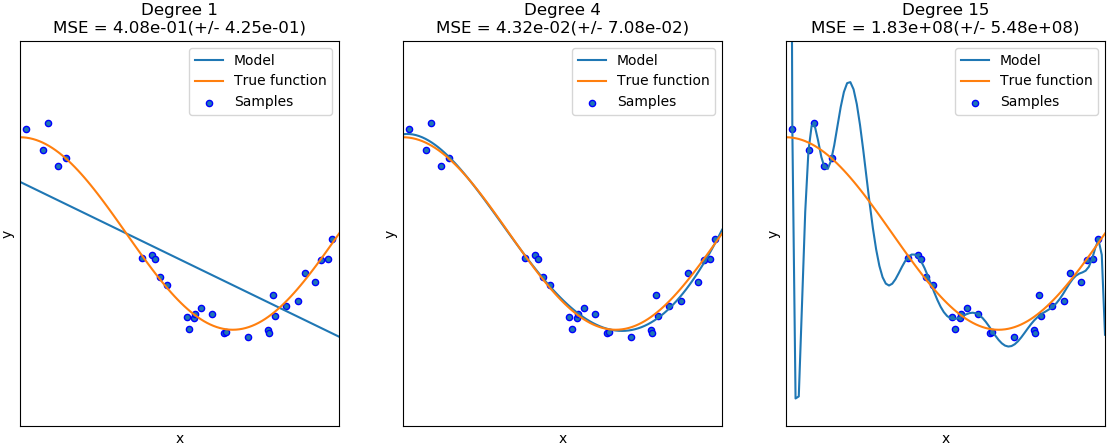
\includegraphics[scale=0.4]{finding-the-perfect-fit.png}
	\captionsetup{labelformat=empty}
	\caption{Esemplificazione tramite simulazione dei fenomeni di \textit{underfitting} e \textit{overfitting}}
\end{figure}


\subsubsection{\textit{Regolarizzazione} e uso dei modelli sovraparametrizzati}

Come abbiamo potuto vedere, la scelta della capacità di un modello può decretarne l'inabilità a modellare dai dati il fenomeno d'interesse, ma anche portarlo ad apprendere gli esempi proposti senza astrarne una relazione significativa, con conseguenze negative per la sua generalizzazione (e di conseguenza applicabilità).

Le due situazioni (\textit{underfitting} e \textit{overfitting}) presentano però una importante asimmetria. Mentre un modello sottoparametrizzato non riuscirà \textit{mai} -- per nessun valore possibile dei suoi pesi -- a modellare il fenomeno d'interesse, un modello sovraparametrizzato ammette -- almeno in teoria -- una o più configurazioni di pesi tali da determinare un modello soddisfacente.

Per questa ragione -- nel caso in cui non si disponga d'informazioni particolari riguardo al fenomeno in esame, non si voglia deliberatamente produrre un modello fortemente approssimato, o \textit{lossy} dai dati o si cerchi il più possibile di preservare il carattere predittivo dello stesso -- la pratica contemporanea del \textit{Machine Learning} preferisce il regime di sovraparametrizzazione dei modelli.

Per contenere gli effetti collaterali conseguenti alla possibilità di \textit{overfitting} e produrre dunque un modello il più possibile simile a quello presentante il numero minimo di parametri necessari (che è però incognito), si può fare uso di opportune \textit{tecniche di regolarizzazione}. Queste possono consistere nella modifica della \textit{loss function} in maniera tale da penalizzare modelli a maggior rischio di \textit{overfitting}, o nell'uso di \textit{priors} opportuni nell'ambito della modellazione Bayesiana, per accennare solo a qualche esempio.

Questo tipo d'approccio non è una novità introdotta in ambito \textit{Machine Learning}: i \textit{penalized likelihood methods}, parte degli approcci statistici tradizionali, si muovono proprio in questa direzione. Come avremo tuttavia modo di analizzare nel seguito, il \textit{Deep Learning} porta all'estremo la sovraparametrizzazione dei modelli utilizzati, con conseguenze tali da richiedere uno studio a parte dei fenomeni che ne derivano.

\subsection{Alcune precisazioni sull'apprendimento supervisionato}

Prima di proseguire il presente lavoro con un'introduzione al \textit{Deep Learning} e alle sue caratteristiche più salienti, può essere utile formalizzare e approfondire alcuni aspetti specifici relativi all'\textit{apprendimento supervisionato}, di gran lunga -- quantomeno allo stato attuale -- il paradigma di \textit{Machine Learning} più diffuso e utilizzato, soprattutto a livello applicativo.

\subsubsection{Descrizione formale}

All'interno del contesto tipico per un problema di \textit{supervised learning} si possono identificare uno \textit{spazio degli input} $\mathbb{I}$, uno \textit{spazio degli output} $\mathbb{O}$ e un \textit{training set}, o \textit{insieme degli esempi} $\mathcal{T} \subseteq \left\{ \mathbb{I} \times \mathbb{O} \right\}$.

Con queste denominazioni, $\mathbb{I}$ rappresenta lo spazio contenente tutte le possibili realizzazioni della codifica scelta per gli input, comprese ovviamente quelle corrispondenti agli input d'interesse sui quali si vorrà applicare il modello appreso al termine del \textit{training}. Lo spazio $\mathbb{O}$, invece, contiene tutte le realizzazioni dei possibili \textit{output}, scelta anche in questo caso una loro opportuna codifica. $\mathcal{T}$ è invece un insieme contenente un numero finito di coppie di \textit{input-output} che si suppongono correttamente associati e da cui di desidera apprendere un modello.

Lo scopo di un algoritmo d'apprendimento appartenente a questa classe è dunque quello di produrre un modello -- appartenente a una famiglia prestabilita e avente iperparametri fissati -- a partire dal solo contenuto di $\mathcal{T}$ e che sia in grado di generalizzare il più possibile su tutta la porzione di $\mathbb{I}$ corrispondente a un fenomeno effettivamente osservabile. Ciò deve avvenire in accordo con il principio di minimizzazione della \textit{loss function} opportunamente scelta $\mathcal{L}$.

Senza perdita di generalità, è possibile assumere che $\mathbb{I}$ e $\mathbb{O}$ siano spazi vettoriali, che $\mathcal{T} = \left\{ \boldsymbol{x}_i, \boldsymbol{\xi}_i \right\}_{i=1}^{n \in \mathbb{N}}$ con $\boldsymbol{x}_i, \boldsymbol{\xi}_i$ vettori di opportuna dimensionalità, che il modello da apprendere abbia la forma $f_{\boldsymbol{w} \in \mathbb{W}, \boldsymbol{h} \in \mathbb{H}}$ con $\boldsymbol{w}$ e $\boldsymbol{h}$ vettori, rispettivamente, dei pesi e degli iperparametri appartenenti a opportuni spazi $\mathbb{W}$ e $\mathbb{H}$. Infine, $\mathcal{L} = \mathcal{L}\left(\left\{ \boldsymbol{x}_i, \boldsymbol{\xi}_i \right\}_{i=1}^{n}, \boldsymbol{w}\right)$.

Il training produrrà quindi un vettore dei pesi stimati $\hat{\boldsymbol{w}}$, da cui il modello stimato $f_{\hat{\boldsymbol{w}}, \boldsymbol{h}}$ sperabilmente in grado di risolvere il problema d'interesse.

\subsubsection{La classificazione}

Quanto detto sinora riguardo all'apprendimento supervisionato si applica con facilità anche al caso della classificazione di \textit{input} opportunamente codificati, in classi di \textit{output} prestabilite e presenti in numero finito.

Per raggiungere tale scopo, è possibile (e vantaggioso) ricorrere allo \textit{one-hot encoding} degli \textit{output} (che rappresentano le varie classi): i vettori $\boldsymbol{\xi}_i \in \mathbb{R}^k$, di dimensione $k$ pari al numero delle classi, sono elementi della \textit{base canonica}, rappresentanti convenzionalmente ciascuno una classe diversa.

La trattazione, a questo punto, è analoga a quella di un qualsiasi problema di \textit{supervised learning}, come già analizzato.


\newpage
\section{Reti neurali artificiali e \textit{Deep Learning}}

Nel panorama del \textit{Machine Learning} contemporaneo -- a livello di ricerca e sviluppo, così come di applicazione -- un ruolo di prim'ordine è senza dubbio ricoperto dal \textit{Deep Learning}, a sua volta evoluzione e raffinamento di principi e tecniche appartenenti all'ambito delle \textit{reti neurali artificiali}, di cui pur fa parte.

Più che un singolo algoritmo, il \textit{Deep Learning} rappresenta un ricco \textit{framework} all'interno del quale formulare e tentare di risolvere i problemi d'apprendimento più vari, appartenenti a ciascuna delle classi delineate in precedenza, sfruttando i medesimi elementi costitutivi che rispondono a un approccio \textit{connessionista} e \textit{statistico-probabilistico} al problema della modellazione matematica e dell'\textit{Intelligenza Artificiale}.

Altro aspetto cruciale di tale metodologia, almeno nella sua concretizzazione moderna, -- e responsabile della sua notevole popolarità -- è la sua vocazione a un trattamento \textit{end-to-end} dei dati: ovverosia alla formulazione automatica e algoritmica di modelli in grado di partire da dati codificati in forma \textit{grezza} (come può essere la sequenza di \textit{bit} con cui un particolare tipo di dato è archiviato digitalmente, o la forma d'onda di un segnale audio), svilupparne una \textit{rappresentazione interna} strutturata e compatta tale da preservarne il contenuto informativo d'interesse, e infine di svolgere su di essa le operazioni necessarie a produrre l'\textit{output} desiderato.


\subsection{Una prospettiva storica}

Nonostante sia stato definito \textit{``Il volto del Machine Learning nel XXI secolo''} (Canziani, 2018), le origini del \textit{Deep Learning} e della modellazione di fenomeni attraverso \textit{reti neurali artificiali} possono essere fatte direttamente risalire ai lavori pionieristici di Rosenblatt (1958), che -- sulla scorta delle proposte formulate nel decennio precedente riguardo la modellazione matematica (deterministica) dei meccanismi assonali e sinaptici del neurone, e dell'apprendimento animale -- per primi si sono posti l'obiettivo di utilizzare tali principi per provare a risolvere un problema concreto, dal punto di vista algoritmico.

Questi approcci, sebbene possano apparire rudimentali e poco efficaci se confrontati con lo stato dell'arte attualmente noto, già contengono tutte le caratteristiche essenziali che saranno ragione del successo di tale paradigma.

\subsubsection{Il Perceptron}

Capostipite di tale famiglia di modelli è il \textit{Perceptron} -- considerabile a tutti gli effetti il \textit{modello neurale artificiale} più semplice e pensato in primo luogo per la risoluzione in contesto supervisionato di problemi ad \textit{input} vettoriale e \textit{output} scalare, discreti, ma facilmente generalizzabile pure al caso continuo.

Utilizzando la notazione già introdotta, il modello in questione produce \textit{output} scalari $y$ a partire da \textit{input} vettoriali $\boldsymbol{x}$ (supposti di dimensione $k$) attraverso una trasformazione affine seguita da una applicazione non lineare $A$, prefissata:

$$
y = A \left( \boldsymbol{x} \cdot \boldsymbol{w} + b \right) = A \left( \sum_{j=1}^{k}{x_j w_j + b} \right)
$$

dove $x_j, w_j$ rappresentano semplicemente le coordinate dei vettori $\boldsymbol{x}, \boldsymbol{w}$ rispetto ad una base scelta (solitamente quella canonica).

%% IMG
\begin{wrapfigure}{r}{0.5\textwidth}
	%\begin{center}
	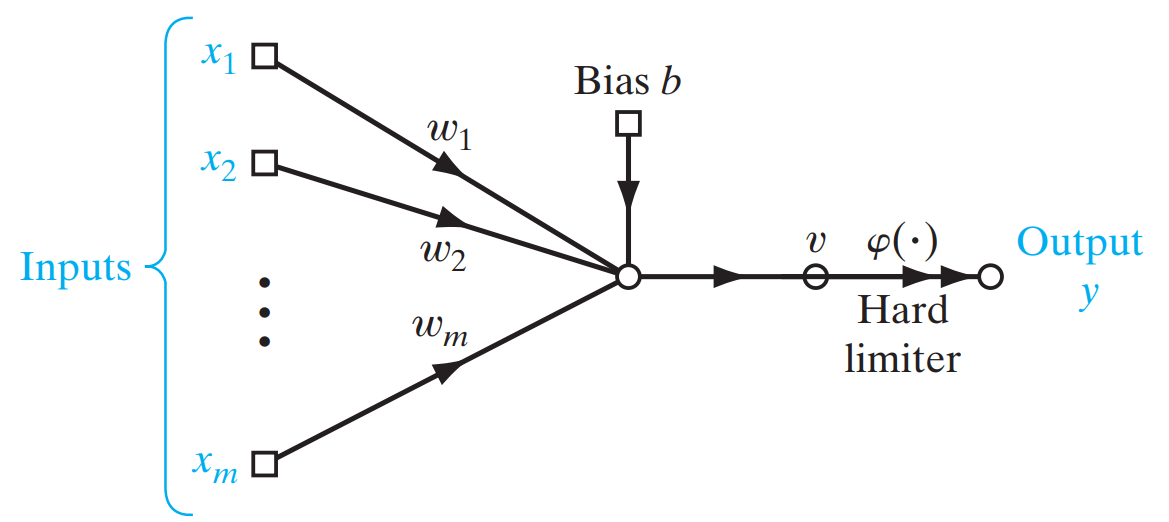
\includegraphics[width=0.94\linewidth]{perceptron.png}
	\captionsetup{labelformat=empty}
	\caption{Possibile rappresentazione di un \textit{Perceptron}.}
	%\end{center}
\end{wrapfigure}

Lo scopo dell'algoritmo d'apprendimento associato al \textit{Perceptron} è dunque quello -- date alcune coppie di esempi di \textit{input-output} considerati corretti, nella forma $\left( \boldsymbol{x}_i, \xi_i \right)$ --  di apprendere i $k+1$ scalari $w_j$ e $b$ che risolvono e generalizzano il problema esemplificato.

Il suddetto algoritmo si articola semplicemente, per ciascuna coppia $\left( \boldsymbol{x}_i, \xi_i \right)$, nell'aggiornare il vettore $\boldsymbol{w}$ e lo scalare $b$ con l'\textit{update step}:

$$
\boldsymbol{w'} \leftarrow \left( \boldsymbol{w} + \epsilon \left( \xi_i - y_i \right) \boldsymbol{x}_i  \right)
$$
$$
b' \leftarrow \left( b + \epsilon \left( \xi_i - y_i \right) \right)
$$

dove $y_i$ è l'output del modello, avente vettore $\boldsymbol{w}$ prima dell'aggiornamento, in corrispondenza all'input $\boldsymbol{x}_i$, e $\epsilon$ uno scalare positivo generalmente minore dell'unità.

Dal parallelo con la neurofisiologia che questo modello e algoritmo associato offrono, hanno origine molti dei termini specifici ancor oggi utilizzati in relazione ai modelli neurali artificiali.

Immaginando idealmente i valori $x_j$ come le intensità di impulsi elettromagnetici condotti dalle sinapsi all'interno di un neurone, i vari $w_i$ prendono il nome di \textit{pesi sinaptici} (o semplicemente \textit{pesi}) e rappresentano all'interno della metafora le quantità di neurotrasmettitore rilasciato nel corpo del neurone alla ricezione del segnale da parte di una specifica sinapsi. Analogamente, $b$ è chiamato \textit{soglia d'attivazione} o \textit{bias}, mentre $A$ \textit{funzione d'attivazione}. Per quanto concerne l'algoritmo di apprendimento, $\epsilon$ è denominato \textit{learning rate} e la descrizione dell'aggiornamento dei parametri è detta \textit{learning rule}.

\subsubsection{Garanzie di convergenza e il problema dell'$ \mathtt{XOR} $}

La pubblicazione della proposta di Rosenblatt fu accolta a suo tempo con notevole entusiasmo e ottimismo per il futuro della disciplina che aveva appena visto la luce -- anche per gli esempi d'applicazione di cui era corredata (come l'apprendimento delle operazioni logiche Booleane $\mathtt{AND}$ e $\mathtt{OR}$) e la prova di un teorema noto come \textit{Perceptron Convergence Theorem}.

Quest'ultimo afferma che, posta l'esistenza di un vettore di pesi $\boldsymbol{\tilde{w}}$ di opportuna dimensionalità e di un \textit{bias} $\tilde{b}$ tali per cui il \textit{Perceptron} associato mappi correttamente tutti i vettori di \textit{input} nell'\textit{output} desiderato, questo terminerà l'apprendimento in un numero finito di \textit{update steps}, a patto di disporre di sufficienti esempi.

Tali problemi, tuttavia, detti \textit{Perceptron-separabili}, si dimostreranno in seguito essere di numero estremamente esiguo rispetto a tutti i problemi d'apprendimento di potenziale interesse. Persino l'operazione logica Booleana $\mathtt{XOR}$ non appartiene a questa classe e la pubblicazione di tale risultato -- che si deve a Minsky \& Papert -- segnerà l'inizio del primo \textit{inverno del connessionismo}.


\subsection{Il \textit{Deep Learning} oggi}

La stagione di scarsa popolarità degli approcci basati su reti neurali artificiali -- e spesso di vera e propria ostilità in seno alla comunità accademica -- si può considerare mitigata a partire dal 1980 con lo sviluppo dell'\textit{algoritmo di backpropagation} ad opera di Hopfield e del \textit{Parallel Distributed Processing Group}. Quindi, definitivamente conclusa nel 2012 con la proposta da parte di Hinton di \textit{ImageNet}, un'architettura neurale profonda in grado di classificare immagini sulla base del loro contenuto con un'accuratezza mai prima raggiunta.

E per quanto, anche alla luce dei risultati ben più sorprendenti riportati in apertura, si fatichi a pensare che corrisponda al vero, la moderna pratica del \textit{Deep Learning} risulta essere fortemente debitrice nei confronti dell'opera di Rosenblatt.

\subsubsection{Lo sviluppo in ampiezza e in profondità}

La differenza principale -- e il motivo di maggior miglioramento nei loro risultati -- dei modelli di \textit{Deep Learning} contemporanei rispetto al \textit{Perceptron} è rappresentato dallo sviluppo \textit{in ampiezza} e \textit{in profondità} evidente nelle architetture moderne.

L'idea all'origine di tale cambiamento d'approccio è ritrovabile in una semplice ipotesi e nelle sue dirette conseguenze. Sapendo che un \textit{Perceptron} è sicuramente in grado di risolvere un problema \textit{separabile}, se un qualunque problema d'apprendimento -- anche non separabile -- fosse scomponibile in un numero finito di sotto-problemi tali da godere di questa proprietà, sarebbe sufficiente utilizzare adeguatamente un certo numero di \textit{Perceptron} distinti per poterlo risolvere.

Al fine di poter proseguire con maggior chiarezza, può essere qui utile introdurre una notazione grafica per rappresentare i \textit{Perceptron}.

Un \textit{Perceptron} (o semplicemente \textit{neurone}) può essere visto come il nodo di un grafo. Tale nodo presenta come proprietà il vettore dei pesi $\boldsymbol{w}$, il \textit{bias} $b$ e la funzione d'attivazione $A$. Con degli \textit{edges} del grafo, generalmente orientati, si rappresentano invece i vari scalari $x_i$ in ingresso nel neurone e l'\textit{output} $y$ in uscita da esso. Un singolo \textit{neurone} sarà quindi descrivibile -- in tale notazione -- come un nodo semplice dotato di alcuni \textit{edges} entranti e uno uscente.

Una moderna architettura neurale artificiale (detta anche \textit{profonda}, per una ragione che sarà immediatamente chiara in seguito) è invece articolata in gruppi di neuroni -- detti \textit{layers} o \textit{strati}, solitamente ordinati -- in linea generale dotati di uguali caratteristiche all'interno del medesimo \textit{layer}, ma differenti altrimenti.

I neuroni del primo strato (detto di \textit{input}) ricevono ciascuno, in ingresso, gli stessi $k$ scalari ${x_j}$, nell'ordine, rappresentabili ugualmente dal vettore $\boldsymbol{x}$ e che costituiscono l'\textit{input} del problema d'apprendimento stesso.

%% IMG
\begin{wrapfigure}{l}{0.5\textwidth}
	%\begin{center}
	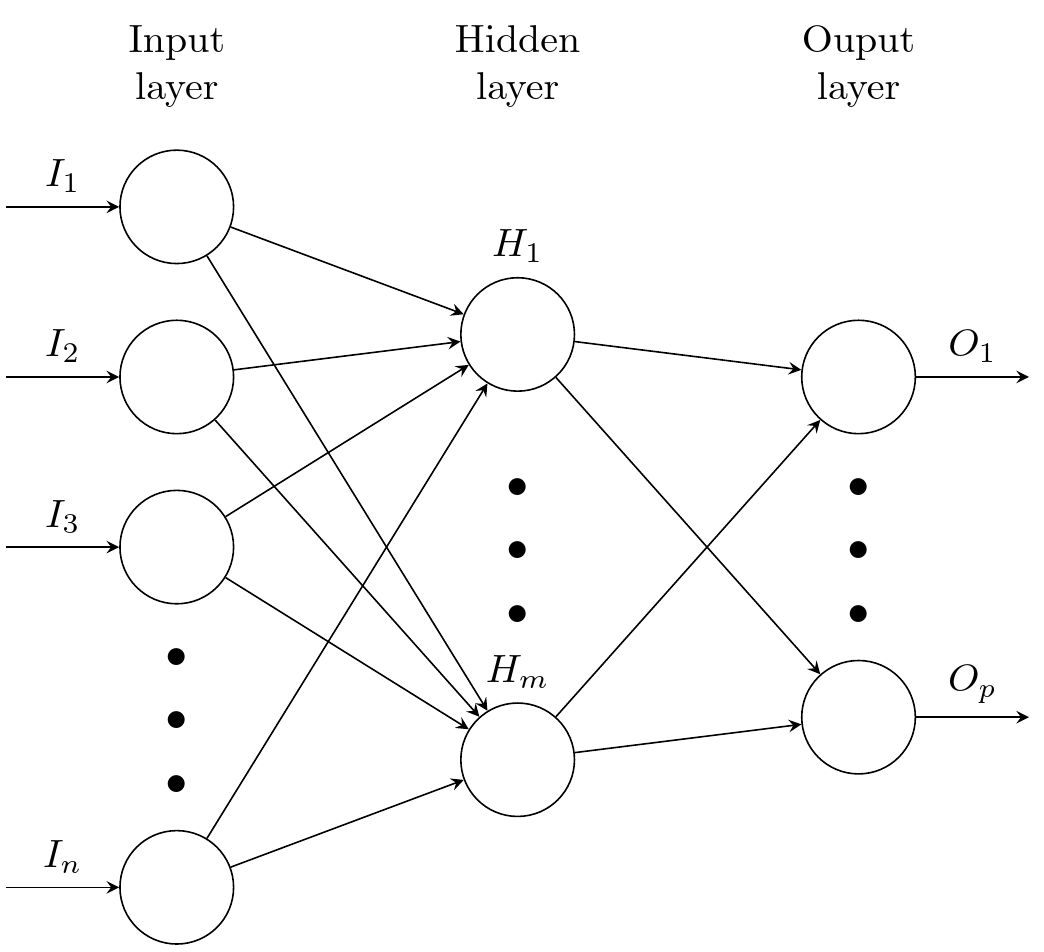
\includegraphics[width=0.94\linewidth]{nnet-graph.png}
	\captionsetup{labelformat=empty}
	\caption{Esempio di grafo associato ad una rete neurale profonda}
	%\end{center}
\end{wrapfigure}

Ciascuno di questi neuroni effettua quindi sull'\textit{input} ricevuto la composizione di trasformazioni prima descritta in relazione al \textit{Perceptron} e la cui $A$ è generalmente la stessa per tutti i neuroni dello strato (non lo sono, invece, i vettori $\boldsymbol{w}$ dei pesi).

Dall'\textit{input layer} -- che consideriamo composto da $l_1 \in \mathbb{N}$ neuroni -- sono così prodotti $l_1$ scalari. Questi possono essere a loro volta considerati le coordinate di un nuovo vettore $l_1$-dimensionale e somministrati una seconda volta in \textit{input} a un nuovo \textit{layer}, iterando il processo un numero di volte arbitrario e coinvolgendovi altrettanti strati di neuroni diversi.

Raggiunto l'ultimo strato di neuroni -- detto \textit{output layer}, a differenza dei precedenti che invece sono denominati \textit{hidden layers} -- il vettore risultante (che può sempre essere uno scalare, nel caso abbia dimensione $1$) può a questo punto essere direttamente utilizzato come \textit{output} del modello o un'ultima volta trasformato da una funzione priva di parametri da apprendere.

La possibilità di poter trasformare l'\textit{input} attraverso un numero $>1$ di neuroni per strato (che definisce l'\textit{ampiezza} del \textit{layer}: i vari $l_1, l_2, ...$) e attraverso numerosi strati in sequenza (il cui numero totale definisce la \textit{profondità} della rete) conferisce una grande capacità di modellazione a questo approccio.

Nell'insieme delle difficoltà che invece interessano simili modelli, va certamente trovato il regime di estrema sovraparametrizzazione a cui è comune ricorrere per evitare di precludersi da principio la corretta risolubilità del problema d'interesse, e l'incremento conseguente di parametri che necessitano di essere appresi -- lineare nel prodotto tra numero di strati e ampiezza media dei \textit{layers}.


\subsubsection{Reti \textit{feedforward} e \textit{fully-connected layers}}

Il tipo di \textit{reti neurali artificiali profonde} sinora descritte, in realtà un sottoinsieme di tutte quelle che possono essere concepite con il formalismo prima introdotto, gode di due precise proprietà, che ne consentono una preliminare classificazione:

\begin{itemize}
	\item {In esso, l'\textit{output} di ciascun neurone costituisce -- al più -- uno degli \textit{input} dei neuroni appartenenti nello strato. Tale assenza di cicli nel grafo o connessioni ad elementi identificati come precedenti (\textit{feedback}) porta a denominare \textit{reti feedforward} tutte quelle che presentano tale caratteristica.\\
	Nel presente lavoro, le suddette saranno l'unico tipo di rete neurale artificiale considerata in relazione a questa suddivisione.}
	\item {Ad eccezione dei neuroni contenuti negli \textit{strati di input} e \textit{output}, tutti gli output costituiscono un \textit{input} per tutti i neuroni del \textit{layer} seguente. Questa proprietà -- riferita in realtà a ciascun singolo \textit{hidden layer} ed estesa all'intera rete -- prende il nome di \textit{connessione totale} e le reti (o i \textit{layers}) che ne godono sono chiamati \textit{fully-connected}}.
\end{itemize}

Motivo del rinnovato interesse nello studio di simili reti neurali artificiali è il cosiddetto \textit{Teorema di Approssimazione Universale}, che in una delle sue tante formulazioni -- associate a rigorose dimostrazioni formali -- afferma che \textit{un qualsiasi problema d'apprendimento -- fornito un numero sufficiente (ma finito) di esempi, e dati un'adeguata profondità (finita) e numero di neuroni per strato (finito) -- può essere correttamente appreso da una rete neurale profonda}.

Il risultato, sicuramente importante, manca tuttavia di un aspetto ritenuto fondamentale nel caso del \textit{Perceptron}: si tratta di un semplice teorema d'esistenza, che non fornisce né garanzie sulla convergenza di un eventuale algoritmo d'apprendimento da applicare a tali modelli, né suggerisce algoritmi pratici per raggiungere il risultato di cui l'esistenza è dimostrata.

La ricerca di simili algoritmi e i risultati sinora ottenuti saranno riassunti nel paragrafo che segue.

Concludiamo riportando una ulteriore possibile formalizzazione del modello sinora descritto, soffermandoci in particolare sul ruolo di un intero \textit{layer} nella trasformazione degli input.

Dato il consueto vettore in ingresso $k$-dimensionale, $\boldsymbol{x}$, uno strato di $l$ neuroni dotato di funzione d'attivazione $A$ agisce su di esso nel modo seguente:

$$
\boldsymbol{y} = A\left(  \boldsymbol{W} \boldsymbol{x} + \boldsymbol{b} \right)
$$

dove $\boldsymbol{x}$ è da intendersi come un vettore \textit{colonna}, $\boldsymbol{W}$ la matrice $l \times k$ avente per righe i vettori dei pesi dei singoli neuroni e $\boldsymbol{b}$ il vettore $l$-dimensionale dei \textit{biases} dei singoli neuroni. Infine, la funzione $A$ è da intendersi applicata elemento per elemento al vettore $\boldsymbol{W} \boldsymbol{x} + \boldsymbol{b}$.

Generalizzando ad un generico strato il formalismo appena introdotto,

$$
L_r(\boldsymbol{x}_r) = A_r\left(  \boldsymbol{W}_r \boldsymbol{x}_r + \boldsymbol{b}_r \right)
$$

e supponendo sempre rispettata la corretta dimensionalità che rende \textit{ben definita} la moltiplicazione matrice-vettore, l'effetto risultante di un'intera rete neurale profonda \textit{feedforward} a $N$ strati su un input $\boldsymbol{x}$ può essere vista come una composizione finita di trasformazioni affini alternate a nonlinearità.

$$
\boldsymbol{y} = Net(\boldsymbol{x}) = L_N( L_{N-1}(\dots (L_1(\boldsymbol{x}))) )
$$


\subsubsection{La discesa lungo il gradiente}

L'algoritmo d'apprendimento (o la vasta famiglia dei tanti, tutti generalmente riconducibili alla medesima trattazione formale) con cui avviene il \textit{training} di una rete neurale profonda è anch'esso assai simile a quello originariamente proposto da Rosenblatt. Una formulazione del suo \textit{update step} è la seguente:

$$
\boldsymbol{\theta'} \leftarrow \boldsymbol{\theta} - \epsilon \boldsymbol{g}
$$

In tal caso, con una differenza rispetto al solito, $\boldsymbol{\theta}$ rappresenta genericamente il \textit{vettore} di tutti i pesi da cui l'intero modello dipende e che si desidera apprendere, mentre $\boldsymbol{g}$ costituisce il gradiente rispetto a $\boldsymbol{\theta}$ -- o una sua approssimazione -- di una \textit{loss function} $\mathcal{L}$ che descriva la bontà del modello appreso sinora.

Affinché suddetta formulazione sia efficace è necessario che $\mathcal{L}$ dipenda da $\boldsymbol{\theta}$ attraverso funzioni differenziabili nei suoi confronti. In generale -- salvo casi particolari che lo richiedano -- la \textit{loss} utilizzata per il \textit{training} di un modello neurale profondo è potenzialmente funzione degli elementi dell'intero \textit{training set} $\mathcal{T}$ e degli \textit{output} del modello stesso prodotti in corrispondenza a \textit{input} opportuni.

Tale dipendenza di $\mathcal{L}$ da $\boldsymbol{\theta}$ attraverso le trasformazioni non lineari descritte dal modello stesso esclude  -- in linea di principio -- l'uso di funzioni $A$ non differenziabili rispetto ai pesi.

Le caratteristiche di $\epsilon$ sono le medesime già enunciate.

La \textit{learning rule} appena esposta, che pur può essere applicata ripetutamente sul medesimo \textit{training set}, costituisce a tutti gli effetti un'iterazione di un algoritmo d'ottimizzazione.

La preferenza per un simile approccio -- confrontato per esempio con strategie di minimizzazione assai più robuste e dalle più solide garanzie analitiche -- può essere spiegata con il carattere fortemente non lineare della trasformazione complessiva che il modello opera sugli \textit{input}, e dal cui \textit{output} $\mathcal{L}$ si trova a dipendere. Inoltre, problema forse ancor più rilevante in tal proposito, la dimensione dello spazio a cui $\boldsymbol{\theta}$ appartiene rende facilmente inapplicabili o inefficaci gli algoritmi di ottimizzazione consueti.

Tale tecnica di ottimizzazione, nell'ambito del \textit{Machine Learning} contemporaneo prende il nome di \textit{discesa lungo il gradiente} o \textit{gradient descent}.

Sicuramente applicabile anche nel caso di spazi ad altissima dimensionalità, tuttavia, il \textit{gradient descent} non è immune a problematiche: per le medesime ragioni poco sopra descritte, l'andamento di $\mathcal{L}$ sul dominio dei $\boldsymbol{\theta}$ presenta molto spesso un notevole numero di minimi locali o \textit{punti a sella} tali da far potenzialmente convergere -- nel caso in cui ciò avvenga -- l'ottimizzatore iterativo in corrispondenza di pesi non ottimali per il modello.

Per quanto, in tale contesto, la sicura convergenza al minimo globale di $\mathcal{L}$ è una proprietà impossibile da garantire, alcune modifiche del \textit{gradient descent} sono state proposte e adottate dalla comunità di ricercatori e professionisti del settore. Una delle prime soluzioni al problema -- da cui originano la gran parte delle successive varianti e raffinamenti -- è nota come \textit{gradient descent with momentum}.

In tal caso -- indicizzando con un pedice gli elementi coinvolti in relazione alle successive iterazioni dell'algoritmo --  contestualmente a ciascun \textit{update} dei pesi è definito un \textit{momento} $\boldsymbol{v}$

$$
\boldsymbol{v}_t \leftarrow \boldsymbol{\theta}_t - \boldsymbol{\theta}_{t-1}
$$

che può essere utilizzato, all'iterazione successiva, per correggere il nuovo aggiornamento:

$$
\boldsymbol{\theta}_{t+1} \leftarrow \boldsymbol{\theta}_{t} - \epsilon \boldsymbol{g}_{t} + \mu \boldsymbol{v}_t
$$

%%
%% IMG
\begin{wrapfigure}{r}{0.5\textwidth}
	%\begin{center}
	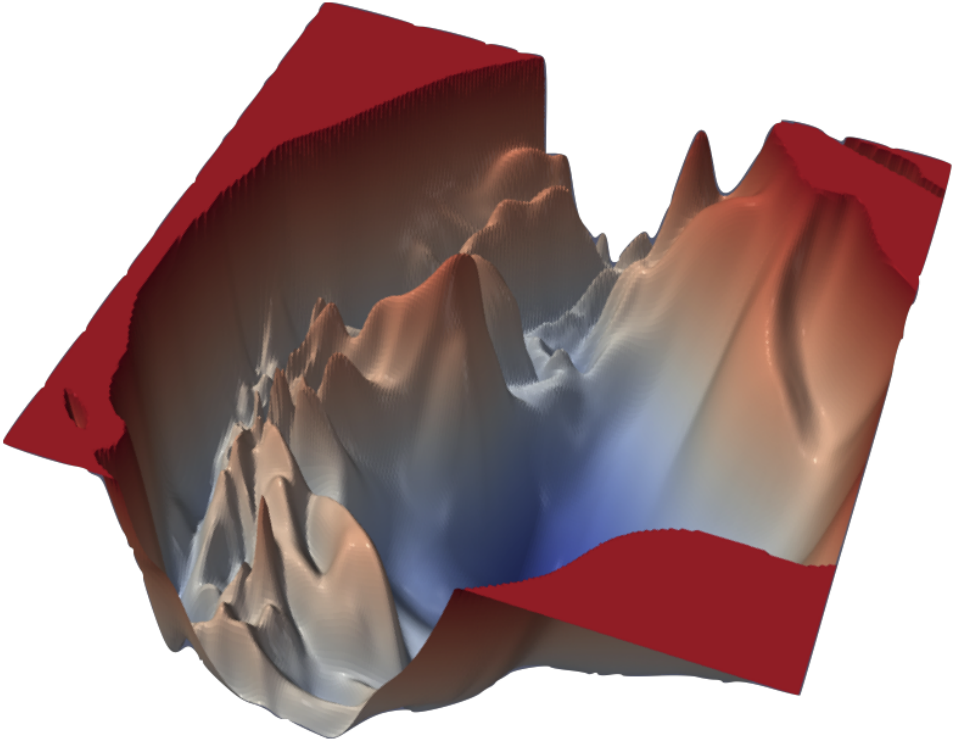
\includegraphics[width=0.94\linewidth]{loss-landscape.png}
	\captionsetup{labelformat=empty}
	\caption{Visualizzazione della dipendenza di $\mathcal{L}$ da due pesi di un modello}
	%\end{center}
\end{wrapfigure}

Il sistema composto da queste due regole d'apprendimento ora espresse in forma implicita può essere esplicitato e utilizzato per fornire all'ottimizzatore un'ulteriore informazione, relativa al percorso seguito subito prima di raggiungere un certo punto nello spazio dei $\boldsymbol{\theta}$, che ne migliora il comportamento al fine d'identificare il minimo globale di $\mathcal{L}$. Costo di questa miglioria è l'introduzione di un nuovo iperparametro, $\mu$.


Più recenti sviluppi in tale direzione sono rappresentati da ottimizzatori -- come \textit{ADAM} o \textit{RMSProp} -- in grado di raccogliere ulteriori informazioni relative alla geometria del \textit{loss landscape} e di sfruttarle per correggere in modo più accurato l'assegnazione iterativa dei nuovi pesi rispetto al semplice termine di discesa lungo il gradiente locale.


\subsubsection{La \textit{Backpropagation}}

Guardando ora all'implementazione degli algoritmi sopra esposti con il fine di derivarne un programma informatico in grado di essere utilizzato nella pratica, il principale ostacolo alla sua efficienza è certamente rappresentato dalla necessità di calcolare un notevole numero di derivate -- una per singolo peso -- a loro volta dipendenti dalla composizione di numerose funzioni.

Una strategia facente uso del principio di \textit{memoizzazione} applicato a suddetto problema è rappresentata dall'algoritmo di \textit{backpropagation}, oggi sfruttato da tutte le librerie \textit{software} che offrano strumenti per in \textit{training} di reti neurali profonde.

Data una generica rete neurale profonda, ricordiamo la struttura della trasformazione complessiva dei suoi \textit{input} in \textit{output}: $\boldsymbol{y} = Net(\boldsymbol{x}) = L_N( L_{N-1}(\dots (L_1(\boldsymbol{x}))) )$.

A questo punto, dovendo calcolare la derivata rispetto a un generico peso $\theta_i$ -- che compare, per ipotesi, tra gli argomenti della funzione $L_{\tilde{s}}$ --  di una \textit{loss function} che dipende esplicitamente dall'output del modello $\mathcal{L}(\boldsymbol{y})$, è possibile andare ad applicare la \textit{regola della catena}.

In tal modo, viene fatta dipendere la derivata $\frac{\partial \mathcal{L}}{\partial \theta_i}$ dalle matrici Jacobiane associate a ciascuna delle funzioni $L$ corrispondenti ai \textit{layers} successivi al $\tilde{s}$-esimo. Vista la necessità di computare il gradiente rispetto a tutti gli elementi di $\boldsymbol{\theta}$, tali matrici associate agli strati dell'intero modello (o addirittura i loro successivi prodotti) possono essere calcolate la prima volta che occorrono, quindi memorizzate, e infine semplicemente riutilizzate in quanto tali nel seguito.

Tale approccio, affinché sia praticabile, richiede pure di disporre -- in una forma algoritmicamente fruibile -- della precisa dipendenza funzionale che lega le varie funzioni $L$ summenzionate ai rispettivi argomenti, e, di conseguenza, ai singoli elementi di $\boldsymbol{\theta}$. Una opportuna struttura ad albero si presta particolarmente a tale scopo e prende il nome di \textit{grafo computazionale}.


\subsection{Il problema della \textit{robustezza}}

I \textit{modelli neurali artificiali profondi}, in virtù della loro notevole e -- almeno in teoria -- arbitrariamente incrementabile capacità, della possibilità che offrono di apprendere trasformazioni \textit{end-to-end}, e grazie alla disponibilità di dati e potenza computazionale oggi ineguagliata rispetto al passato, sono ormai diventati la scelta primaria per alcune attività di modellazione statistica, nonché componente essenziale di applicazioni parte della vita quotidiana di molte persone.

Basti pensare, a tal proposito, ai sistemi di riconoscimento facciale o vocale con cui è possibile sbloccare un dispositivo digitale, ai meccanismi di assistenza alla guida che avvisano il conducente di un veicolo della presenza di un determinato segnale stradale o che attivano il sistema frenante della vettura nel caso di un ostacolo imprevisto.

Tale versatilità dei sistemi di \textit{Deep Learning}, unita a una ottima efficacia nella gran parte dei loro utilizzi pratici, potrebbe indurre credere -- ingenuamente -- che tali sistemi, pur presentando delle debolezze tipiche di tutti i sistemi d'apprendimento statistico, non possano essere soggetti a errori \textit{catastrofici}, tali cioè da precluderne completamente l'applicabilità in un determinato ambito.

A tale proposito, può essere interessante analizzare il problema della \textit{robustezza} dei classificatori neurali profondi.

\subsubsection{I classificatori e la loro accuratezza}

Considerando il tipico scenario associato a un problema di classificazione supervisionato -- indipendentemente dal tipo di modello e di algoritmo d'apprendimento utilizzato -- è sempre possibile formulare la soluzione del problema in esame come la capacità del modello prodotto di associare un qualunque \textit{input} su cui potenzialmente s'intende utilizzare il classificatore alla classe di \textit{output} che si ritiene corretta per tale \textit{input}.

Per questa ragione, una comune misura della bontà di un classificatore è la sua \textit{accuratezza}, valutata su di un \textit{test set}.

Questo corrisponde a selezionare una serie di esempi rappresentativi dello specifico caso d'uso del classificatore -- in generale non utilizzati in fase di \textit{training} -- e calcolare il rapporto tra il numero d'esempi classificati correttamente e il loro totale.

La metrica di \textit{accuratezza} appena definita è solitamente utilizzata come indicatore per la selezione -- tra vari modelli già allenati -- del classificatore più adatto a svolgere un dato compito, o come misura della bontà della propria soluzione applicativa rispetto a quelle proposte dai concorrenti commerciali.

Questo tipo d'indicazione, tuttavia, non è in grado di cogliere un aspetto che può rivelarsi cruciale in quelle situazioni dove un errore di classificazione potrebbe rivelarsi non tollerabile -- specie se prodotto da un \textit{avversario} interessato a provocare un malfunzionamento nel classificatore: la \textit{robustezza}.


\subsubsection{Robustezza e \textit{Manifold Hypothesis}: un'intuizione geometrica}

Un punto di partenza per comprendere il significato intuitivo del concetto di \textit{robustezza} -- essendo una rigorosa trattazione geometrica dello stesso al difuori degli obiettivi del presente lavoro -- è offerto dalla cosiddetta \textit{Manifold Hypothesis}, proposta di recente (Dube et al., 2018) all'interno di un più vasto insieme di tentativi volti a fornire di fondazioni più rigorose e analiticamente trattabili una serie di problematiche osservate già da tempo in relazione ai modelli neurali profondi.

Innanzitutto, è necessario sottolineare il fatto che un qualunque classificatore, tale, al termine del training, da accettare un \textit{input} codificato secondo un opportuno \textit{input coding} per associarlo alla corretta classe di \textit{output} tra quelle possibili, eseguirà una simile classificazione per qualunque \textit{input} consentito dalla codifica scelta, indipendentemente dal fatto che questo sia o meno ritenuto \textit{di interesse} per un eventuale utente dello stesso o espressione di un fenomeno \textit{naturale}.

Immaginando quindi -- all'interno dello spazio offerto da tale codifica (e detto semplicemente \textit{input space}) -- di considerare ogni possibile \textit{input} processabile da un certo classificatore, è possibile suddividere suddetto spazio in regioni, gli elementi di ciascuna delle quali sono mappati nella medesima classe di \textit{output}. I punti dell'\textit{input space} tali da separare regioni diverse costituiscono l'insieme delle \textit{decision boundaries} del classificatore studiato.

%%%
%\begin{figure}[H]
%	\centering
%	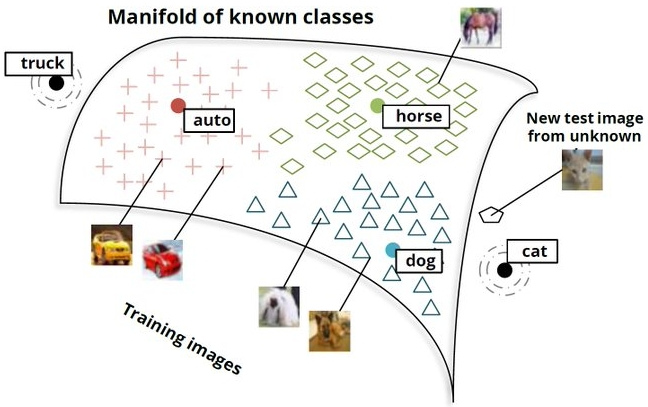
\includegraphics[scale=0.4]{manifold-hyp.jpeg}
%	\captionsetup{labelformat=empty}
%	\caption{Esemplificazione tramite simulazione dei fenomeni di \textit{underfitting} e \textit{overfitting}}
%\end{figure}


\begin{wrapfigure}{l}{0.5\textwidth}
	%\begin{center}
	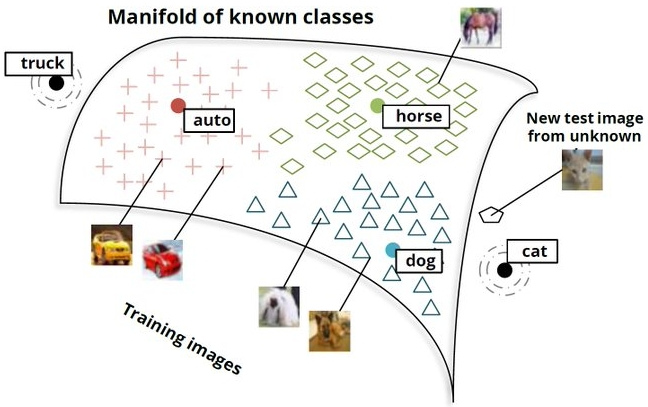
\includegraphics[width=0.94\linewidth]{manifold-hyp.jpeg}
	\captionsetup{labelformat=empty}
	\caption{Una rappresentazione informale ma intuitiva della \textit{Manifold Hypothesis}}
	%\end{center}
\end{wrapfigure}


La \textit{Manifold Hypothesis} asserisce dunque che i dati in \textit{input} associati ai casi considerati d'interesse, o analogamente utilizzati in fase di \textit{training} o per il computo dell'accuratezza di un classificatore, si possano assumere come appartenenti a una varietà (\textit{data manifold}) immersa nell'\textit{input space} e avente dimensione anche molto minore di esso. Le \textit{decision boundaries}, di conseguenza, sarebbero anch'esse ipersuperfici immerse nello spazio degli input, le cui intersezioni con il \textit{data manifold} vengono apprese a partire dagli esempi forniti.

Nel \textit{framework} così descritto, quindi, i possibili \textit{input} in grado di determinare un comportamento non previsto nel classificatore sono raggruppabili in due categorie:

\begin{itemize}
	\item {Quelli che, pur rappresentando \textit{input} di potenziale interesse per l'uso del classificatore -- e quindi appartenenti al \textit{data manifold} o in sua vicinanza -- sono prossimi ad una \textit{decision boundary} e collocati in una regione considerata non corretta;}
	\item {Quelli che, non facenti parte del \textit{data manifold}, non rappresentano \textit{input} d'interesse, ma ugualmente vengono classificati dal modello proposto}.
\end{itemize}

A livello intuitivo, la \textit{robustezza} di un classificatore è una misura della suscettibilità dello stesso a manifestare il comportamento (non previsto) appena descritto.

\subsubsection{\textit{Adversarial attacks} ed $\epsilon$-robustezza}

Nella descrizione del fenomeno che stiamo trattando, gli elementi dell'\textit{input space} facenti parte delle due categorie sopra elencate prendono generalmente il nome di \textit{adversarial examples} per il classificatore considerato. Procedure sviluppate con lo scopo di produrre \textit{adversarial examples} -- noto che sia il classificatore di cui cercare una vulnerabilità -- vengono denominate \textit{attacchi}.

Tra le due categorie di \textit{adversarial examples} sopra descritte, la prima ricopre certamente un ruolo di maggior rilievo. La possibilità di incontrare in corso d'utilizzo -- o addirittura di produrre ad arte -- specifici \textit{input} che, pur annoverati tra quelli d'interesse, possano essere classificati in maniera inadeguata da un modello è infatti un aspetto a cui prestare particolare attenzione nel caso -- ormai già citato più volte -- in cui si voglia certificare non solo l'accuratezza, ma pure la \textit{sicurezza d'uso} di un classificatore o di un'applicazione che da esso dipende.

Una misura rigorosa della robustezza a tale tipo d'attacchi per un classificatore è, ad esempio, l'$\epsilon$-robustezza, che può essere formalizzata nel modo che segue.

Sia dato un classificatore $C$ che opera sullo spazio $k$-dimensionale degli input  $\mathbb{I}$ e produce in \textit{output} una variabile categorica rappresentante una classe a cui l'\textit{input} appartiene. Siano dati inoltre un esempio $\boldsymbol{x} \in \mathbb{I}$, un generico vettore $\boldsymbol{p}$ tale che sia definita l'oprazione di somma $\boldsymbol{x} + \boldsymbol{p}$ e uno scalare $\epsilon$.

Si dirà dunque che $C$ è un classificatore $\epsilon$-robusto in $\boldsymbol{x}$ rispetto alla norma $|| \cdot ||$ se:

$$
\forall \boldsymbol{p} \ \text{t.c.} \ ||\boldsymbol{p}|| < \epsilon, \ C(\boldsymbol{x}) = C(\boldsymbol{x} +\boldsymbol{p} )
$$

Similmente, un \textit{attacco $\epsilon$-perturbativo in $\boldsymbol{x}$ rispetto alla norma $|| \cdot ||$} sarà una procedura atta a trovare un vettore $\boldsymbol{p}$ che, rispettando la condizione $||\boldsymbol{p}|| < \epsilon$ determina la disuguaglianza $C(\boldsymbol{x}) \neq C(\boldsymbol{x} +\boldsymbol{p} )$.

Anche qualora non si consideri la possibilità che un \textit{avversario} abbia l'interesse, la volontà o le risorse necessarie per sferrare un \textit{attacco} contro un certo classificatore, la pratica di valutarne la \textit{robustezza} contro \textit{attacchi $\epsilon$-perturbativi} può rappresentare un'occasione per testarne la validità nei confronti di \textit{input} imprevisti o per indagare le proprietà delle sue \textit{decision boundaries}.

In generale, gli \textit{attacchi \textit{adversarial}} possono essere classificati in base alla quantità d'informazioni che l'\textit{attaccante} è in grado di conoscere riguardo al modello che dev'essere attaccato. Un'altra possibilità, invece, considera l'effetto che l'attacco dovrà sortire sul classificatore.\\
Nel caso in cui il modello sia completamente accessibile (compresi \textit{loss function} utilizzata in fase di \textit{training}, valori dei pesi e degli iperparametri, architettura del modello, ...) si parlerà di attacco \textit{white-box}. Viceversa, se l'attaccante è solamente in grado di valutare il modello in corrispondenza di determinati \textit{input}, si avrà a che fare con un attacco \textit{black-box}. La situazione è tuttavia più sfumata: alcuni attacchi, ad esempio, possono addirittura disporre del \textit{training set} esatto che è stato utilizzato per allenare un certo classificatore.\\
Sul fronte dei risultati prodotti, invece, un attacco si dirà \textit{targeted} quando ha lo scopo di spingere il modello a classificare (in maniera errata) un esempio come appartenente ad una classe specifica. Si dirà invece \textit{untargeted} quando il successo dell'attacco non dipende dall'\textit{output} prodotto (purche, come sempre, non sia quello corretto).

\subsubsection{Un esempio: \textit{PGD Attack}}

A titolo d'esempio -- e poiché sarà utile nel seguito --, riportiamo qui la breve descrizione di un attacco iterativo \textit{white-box}, particolarmente efficace e adattabile a qualsiasi norma scelta, che sfrutta il principio di \textit{gradient descent} precedentemente introdotto: \textit{Projected Gradient Descent Attack}.

Nella sua formulazione \textit{untargeted}, l'algoritmo che lo descrive è estremamente breve. Scelto un qualsiasi input che si è sicuri venga classificato correttamente dal modello attaccato, si costruisce la palla chiusa di raggio $\epsilon$ -- con metrica indotta dalla norma considerata -- centrata in esso.

Quindi, iterativamente e con \textit{update steps} identici a quelli descritti per identificare i pesi più adatti per un dato modello, si ottimizza invece nello spazio degli \textit{input} con una \textit{loss} opposta a quella del classificatore considerato.

Nel caso, a seguito di un \textit{update}, l'elemento considerato nello spazio degli \textit{input} si trovi al di fuori della palla precedentemente costruita, sarà sufficiente proiettarlo sulla sua frontiera prima dell'iterazione successiva.

%% IMG
\begin{figure}[H]
	\centering
	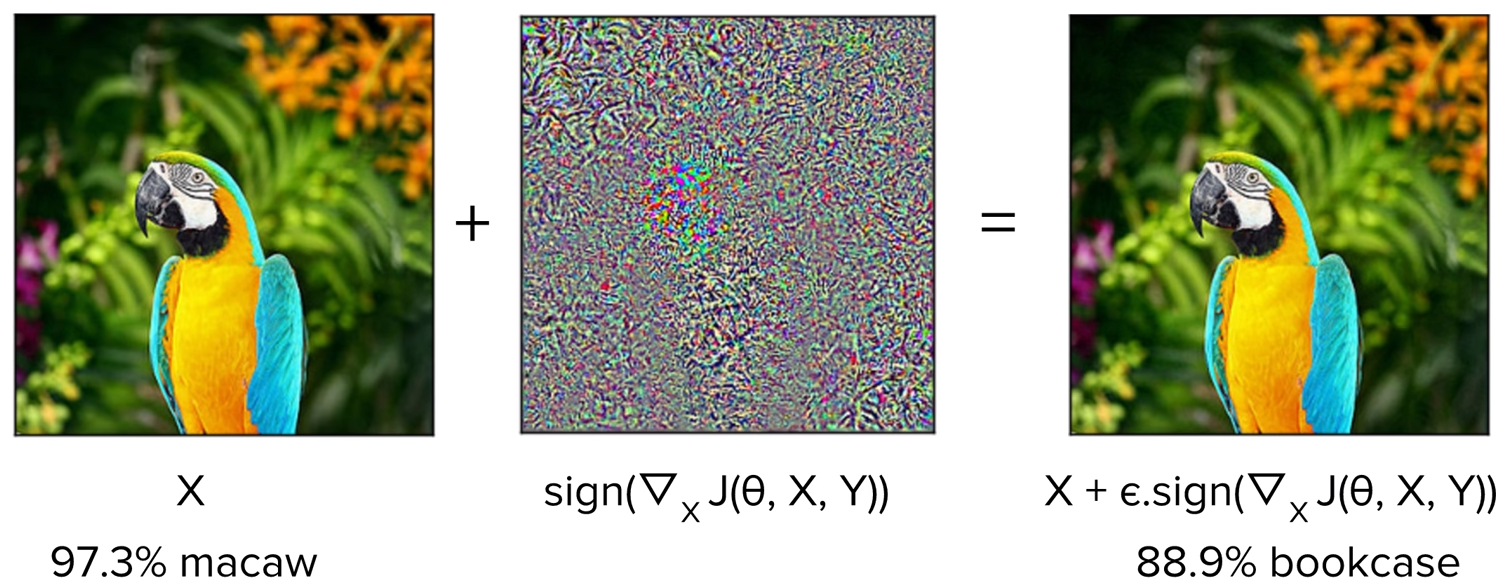
\includegraphics[scale=0.4]{fgsm-macaw-bookcase.png}
	\captionsetup{labelformat=empty}
	\caption{Esemplificazione di un adversarial attack simile a quello descritto (FGSM); in tal caso è utilizzata solo l'informazione sul gradiente della loss. L'immagine risultante è visivamente indistinguibile da quella iniziale, non soltanto al fine di classificazione. }
\end{figure}

\subsubsection{Cenni: Relative difese}

Così come per la generazione di \textit{attacchi}, numerosi metodi sono stati proposti per difendersi da questi. Senza scendere negli aspetti più tecnici, la grandissima parte di tali \textit{difese} è basata sul principio di \textit{adversarial training} o sue varianti.

Nella sua forma più semplice, dato un certo classificatore già allenato e la possibilità di generare attacchi -- in linea di principio di qualunque tipo -- contro di esso, si tratta di proseguire semplicemente il \textit{training} del classificatore su un \textit{dataset} composto da quello originale arricchito dei risultati prodotti da suddetti \textit{attacchi}.

In generale, tuttavia, anche le tecniche più avanzate in tal senso non mettono in discussione quella che pare essere un'assunzione di fondo: l'apprendimento dei pesi di un \textit{classificatore neurale profondo} deve avvenire tramite \textit{gradient descent} a partire da una \textit{loss function} dipendente dal suo output e i cui \textit{update steps} sono computati attraverso \textit{backpropagation} sul modello stesso.

Da tale osservazione è nata l'idea -- in controtendenza -- che è proposta nel capitolo che segue.


\newpage
\section{Modelli generativi dei pesi e \textit{adversarial attacks}}

Il presente capitolo, ben lungi dal voler costituire una trattazione completa e definitiva dell'argomento, ha lo scopo di descrivere l'esplorazione preliminare -- e i risultati che questa ha sinora determinato -- dell'approccio a cui si è alluso in conclusione della sezione precedente: l'utilizzo di un \textit{deep neural model} generativo, associato ad uno specifico protocollo di \textit{training}, per la determinazione diretta dei pesi di un classificatore. Nel dettaglio, particolare attenzione è stata posta alla questione di verificare preliminarmente se tale percorso potesse rivelarsi di qualche utilità allo scopo di migliorare la robustezza di suddetto classificatore, o di consentire un adattamento del \textit{tradeoff} tra accuratezza e robustezza (caratteristica che si verifica solitamente come conseguenza dell'\textit{adversarial training}) senza necessitare del \textit{re-training} dell'intero modello.


\subsection{Caso d'uso e pre-requisiti}

Il modello generativo, e associato protocollo di \textit{training}, proposti sono stati concepiti per l'utilizzo in un contesto nel quale si disponga:

\begin{itemize}
	\item {Di un \textit{classificatore neurale profondo}, già allenato, il cui \textit{training} si sia svolto senza tenere in considerazione il problema della \textit{robustezza};}

	\item {Del \textit{training set} su cui suddetto allenamento sia stato praticato, o -- in generale -- di un \textit{training set} rappresentativo del problema d'interesse;}

	\item {Della possibilità di provare a generare \textit{adversarial examples $\epsilon$-perturbativi} per qualunque elemento di suddetto \textit{dataset} -- anche senza successo -- soddisfacendo in tal senso ogni ulteriore requisito la metodologia d'\textit{attacco} scelta (unica) richieda;}

	\item {Della possibilità di valutare il modello su un qualunque \textit{input} consentito dal \textit{coding} scelto;}

	\item {Dell'accesso, in qualunque momento, al valore dei pesi del classificatore.}

\end{itemize}

Tali condizioni, in generale, si può supporre che siano verificate nel caso in cui l'ipotetico utente della procedura proposta sia il medesimo responsabile del suo \textit{training} e -- per tale ragione -- sia potenzialmente interessato a valutarne e migliorarne le proprietà di robustezza.

Risultato dell'applicazione di tale proposta è un modello dotato della stessa architettura e del medesimo numero di parametri rispetto a quello originariamente disponibile.

Infine, è bene sottolineare come la procedura proposta non sfrutti in alcun modo esplicito l'eventuale struttura del modello già disponibile, essendo così applicabile in linea di principio a qualunque architettura.


\subsection{Descrizione del modello generativo e della procedura di \textit{training}}

Prima di proseguire con la trattazione del principale argomento del presente paragrafo, è utile introdurre una ulteriore specifica misura di robustezza.

\subsubsection{\textit{Empirical Global Robustness}}

Siano fissati un classificatore già allenato, il \textit{training dataset} su cui tale allenamento sia avvenuto o -- equivalentemente -- un \textit{dataset} d'interesse su cui ci si aspetta di osservare un'accuratezza confrontabile, un generatore d'\textit{attacchi} $\epsilon$-perturbativi, di qualunque tipo, utilizzabile sul classificatore suddetto e un valore di $\epsilon$.

Poste tali condizioni, e un numero naturale $N$, da cui questo valore dipende, la \textit{empirical global robustness} è il rapporto tra il numero di attacchi falliti sul totale degli $N$ elementi del \textit{dataset} perturbati.

Avendo tale stimatore le medesime caratteristiche di una \textit{media campionaria}, ci si può aspettare che tale valore sia tanto più rappresentativo della reale \textit{$\epsilon$-robustezza} media del classificatore su tutti gli \textit{input} d'interesse tanto più $N$ sia prossimo al totale degli elementi del \textit{dataset} disponibile e tanto più quest'ultimo sia effettivamente rappresentativo del problema in esame.

\subsubsection{Architettura del modello e ruolo delle rispettive parti}

Il modello generativo proposto si compone di due \textit{parti}, entrambe reti neurali profonde: un \textit{generatore di pesi} $\mathcal{G}$ e un \textit{value network} $\mathcal{V}$.

In breve -- all'ipotetica conclusione del rispettivo \textit{training} -- lo scopo di $\mathcal{G}$ è quello di mappare del rumore campionato da uno spazio $z$-dimensionale in un vettore di $q$ scalari ordinati che andranno a costituire dei pesi (sperabilmente presentanti le proprietà desiderate) per il classificatore inizialmente disponibile. Quello di $\mathcal{V}$ è invece di stimare, direttamente dai valori delle coordinate dei pesi ($\boldsymbol{\theta}$, logicamente un vettore $q$-dimensionale) l'accuratezza e la \textit{empirical global robustness} del classificatore considerato.

L'unica proprietà che è esplicitamente richiesto sia posseduta da $\mathcal{V}$ è la differenziabilità del suo \textit{output} rispetto all'\textit{input}: una caratteristica solitamente associata con una conseguenza della sua stessa allenabilità.

Tale ultima richiesta è collegata all'intenzione di utilizzare proprio una funzione dell'\textit{output} di $\mathcal{V}$ come \textit{loss function} per l'allenamento di $\mathcal{G}$.

La scelta -- apparentemente bizzarra -- di una simile architettura per un modello generativo dipende da una rielaborazione dei risultati sui modelli generativi con \textit{loss} dipendente da un modello discriminativo (Goodfellow 2013 e 2014), culminati nella definizione dei \textit{Generative Adversarial Networks}, e dall'uso che viene fatto dei \textit{value networks} in \textit{Reinforcement Learning} per l'approssimazione differenziabile di funzioni non differenziabili (tra cui -- a titolo d'esempio -- Sabatelli, 2018).

\subsubsection{Dinamica di \textit{training}}

Nel corso dell'allenamento del modello sin qui descritto, un singolo \textit{training step} è composto dalle seguenti parti, in ordine:

\begin{enumerate}
	\item Un vettore aleatorio reale $\boldsymbol{s}$ di dimensione $z$ è campionato da una distribuzione nota;
	\item Viene calcolato il vettore $q$-dimensionale $\mathcal{G}(\boldsymbol{s}) = \boldsymbol{\theta}$;
	\item I pesi del modello discriminativo inizialmente noto sono sostituiti dalle componenti del vettore $\boldsymbol{\theta}$, in un ordine prefissato;
	\item Il classificatore così costruito viene valutato sugli elementi del \textit{training set} fornito, o su un suo sottoinsieme al fine di calcolarne l'accuratezza $\mathfrak{A}$;
	\item Il medesimo classificatore viene attaccato con un attacco prefissato -- su ciascun elemento dell'insieme adoperato per il calcolo dell'accuratezza -- e viene calcolata la \textit{empirical global robustness} $\mathfrak{R}$ così ottenuta;
	\item Viene calcolato il vettore delle stime di \textit{accuratezza} e \textit{global adversarial robustness} $(\hat{\mathfrak{A}},\hat{\mathfrak{R}}) = \mathcal{V}(\boldsymbol{\theta})$;
	\item È eseguito l'\textit{update} dei pesi di $\mathcal{V}$ sulla base di una metrica di similarità tra $(\hat{\mathfrak{A}},\hat{\mathfrak{R}})$ e $({\mathfrak{A}},{\mathfrak{R}})$
	\item È eseguito l'\textit{update} dei pesi di $\mathcal{G}$ usando come \textit{loss} una funzione della forma $$\mathcal{L}(\boldsymbol{\theta}) =  -\alpha \hat{\mathfrak{A}}(\boldsymbol{\theta}) - \beta \hat{\mathfrak{R}}(\boldsymbol{\theta})$$ dove $\alpha + \beta = 1$ (o una qualunque altra costante).
\end{enumerate}

\subsubsection{Alta dimensionalità di $\boldsymbol{\theta}$ e \textit{pretraining}}

A livello teorico, il protocollo di \textit{training} sopra introdotto potrebbe già essere capace di produrre risultati d'interesse per il modello proposto.

Tuttavia, il fatto che la dimensione di $\boldsymbol{\theta}$ sia pari al numero totale di pesi di un altro modello neurale profondo (e quindi generalmente nell'ordine di grandezza delle centinaia di migliaia anche per problemi multi-classe relativamente semplici) rende la convergenza di una simile procedura estremamente lenta, inaccurata o -- nella maggior parte dei casi -- ragionevolmente impossibile. Ciò è ulteriormente aggravato dal fatto che entrambi i modelli $\mathcal{G}, \mathcal{V}$ dipendono ciascuno direttamente dal vettore $\boldsymbol{\theta}$, ma la convergenza di $\mathcal{G}$ lo fa anche attraverso la \textit{loss} stimata da $\mathcal{V}$.

Per cercare di aggirare questo ostacolo, riuscendo in tal modo pure ad integrare la \textit{prior knowledge} proveniente dall'aver già allenato un classificatore tale da massimizzare l'accuratezza per il problema d'interesse, si può fare ricorso al \textit{pre-training} di $\mathcal{G}, \mathcal{V}$.

Tale denominazione denota una procedura di \textit{training} non finalizzata ad apprendere il modello desiderato, ma tale da facilitarne in un secondo momento l'apprendimento vero e proprio.

Secondo una strada già percorsa da Bengio (2008), Hinton (2012), ma anche più recentemente Howard \& Gugger (2017), la tipologia di \textit{pre-training} qui adottata mira a portare il modello in regime di \textit{overfitting} rispetto ad un numero esiguo di esempi con il solo scopo di conferire ai suoi pesi una struttura che si assume essere euristicamente simile a quella del modello ipoteticamente appreso senza \textit{pre-training} nelle fasi terminali dell'apprendimento.

Il modello associato a $\mathcal{G}$ può essere allenato in tal senso anche con il solo esempio costituito dai pesi del modello inizialmente fornito, in output, associato ad un \textit{input} fissato (ad esempio la media della distribuzione da cui $\boldsymbol{s}$ è campionato).

Quello associato a $\mathcal{V}$, analogamente, con i pesi del modello inizialmente fornito, in \textit{input}, e i suoi valori effettivi di $({\mathfrak{A}},{\mathfrak{R}})$ in output.

Per la medesima ragione, anche nelle fasi iniziali della \textit{dinamica di training} sopra descritta, il vettore $\boldsymbol{s}$ può essere campionato da una medesima distribuzione con parametri di dispersione (qualora essa ne sia provvista) crescenti con il numero di iterazioni fino al raggiungimento del valore massimo desiderato -- controllando euristicamente in tal modo la massima variazione dell'output di $\mathcal{G}$.

\subsubsection{Sulla necessità dell'uso di $\mathcal{V}$}

Viste le notevoli complicazioni che ciò comporta, si potrebbe dubitare della sensatezza dell'uso di una \textit{value function} nella stima della \textit{training loss} desiderata per $\mathcal{G}$.

La risposta più immediata a tale potenziale obiezione è sicuramente legata alla generale non-differenziabilità rispetto ai pesi di $\mathcal{G}$ delle funzioni $({\mathfrak{A}},{\mathfrak{R}})$ che s'intendono utilizzare.

Vi sono tuttavia due ulteriori motivazioni, più profonde, tali da giustificarne l'uso. La prima -- legata al computo di una metrica di robustezza -- è rappresentata dalla generale assenza di differenziabilità nei confronti di $\boldsymbol{\theta}$ delle procedure (solitamente iterative e nemmeno continue) che portano alla generazione di un \textit{adversarial example}. La seconda -- invece di natura tecnica e collegata al computo di una metrica di accuratezza -- è costituita dalla comune scelta implementativa delle più robuste librerie di \textit{Deep Learning} disponibili, come quella utilizzata nella fase \textit{sperimentale} descritta nel seguito, di non consentire la differenziazione attraverso le operazioni di sovrascrittura dei pesi -- come quella descritta nella \textit{dinamica di training} sopra riportata.


\subsubsection{Sulla scelta di non utilizzare \textit{batching} o regolarizzazioni}

Prima di procedere con la descrizione delle procedure sperimentali volte all'indagine delle proprietà del modello proposto, è utile riportare una breve nota riguardo alle ragioni per cui -- all'interno delle procedure descritte in precedenza -- non è mai stata menzionata la possibilità di ricorrere a strategie di regolarizzazione, pur presenti anche dell'ambito del \textit{Deep Learning}. Di analoga giustificazione è inoltre il motivo per cui nella \textit{dinamica di training} sopra riportata non viene fatto utilizzo del \textit{batch training} -- ovverosia della comune pratica, capace di velocizzare la convergenza della discesa lungo il gradiente, di \textit{accumulare} in forma mediata o sommata i gradienti rispetto ai pesi di un modello per alcune iterazioni, prima di eseguire l'\textit{update step} effettivo.

La ragione di tali scelte è da cercarsi nei risultati di Madry (2017): tutte le procedure descritte hanno come effetto -- collaterale o voluto -- la modifica della distribuzione dei valori dei pesi all'interno dei \textit{layers} (compreso quello di \textit{output}) del modello su cui sono applicate. Alcune di tali informazioni, tuttavia, sono generalmente considerate un buon indice indiretto riguardo alla robustezza di un modello. Per tale ragione -- anche a costo di rallentare la convergenza dei modelli indagati -- si è preferito evitare di alterarne in contenuto informativo in tal senso.

\subsection{Indagine sperimentale}

Nella formulazione del modello e del \textit{protocollo di training} descritti in precedenza, non è mai stato fatto esplicito riferimento ad un ambito preferenziale d'applicazione dello stesso, o a specifiche architetture per l'implementazione di $\mathcal{G}$ e $\mathcal{V}$, o anche a particolari \textit{adversarial attacks} da utilizzare in fase di \textit{training}.

Questo, oltre che alla totale generalità con cui la presente proposta può essere adattata ai diversi contesti con il fine di analizzarne il comportamento, dipende dal fatto che -- essendo modello e protocollo di \textit{training} formulazioni originali e ancora in fase d'indagine preliminare -- non sono generalmente disponibili informazioni tali da consentire d'identificarne gli ambiti di più proficua applicazione.

Questo, tuttavia, non ha impedito di provare a testare quanto proposto su un \textit{toy problem} con finalità esplorative.

\subsubsection{Il dataset: \textit{MNIST}}

Il \textit{dataset} utilizzato per tale \textit{test run} è costituito da \textit{MNIST}. Si tratta della raccolta di $10000$ immagini in \textit{bianco e nero}, quadrate e di lato pari a $28$ pixel, raffiguranti le cifre arabe dallo $0$ al $9$ in diverse grafie manoscritte.

Lo scopo di un eventuale classificatore per tale problema consiste nell'associare ciascuna immagine al corretto \textit{one-hot vector} corrispondente alla rappresentazione di ciascuna cifra.

Il problema è generalmente considerato -- attualmente -- di facile risoluzione per quanto riguarda l'accuratezza del classificatore appreso.

L'\textit{input coding} utilizzato, ormai considerato standard per tale \textit{dataset}, è costituito dalla trasformazione dei $784$ pixel in un vettore ordinato, nell'assegnazione del valore $0$ al colore nero e $1$ a quello bianco (o viceversa) e infine dalla normalizzazione del valore associato a ciascun pixel per una costante dipendente dal modello adoperato. Quest'ultimo \textit{step} può essere omesso, dal momento che è solo utile a velocizzare il \textit{training}.

\subsubsection{Il classificatore: \textit{LeNet5}}

Il classificatore pre-allenato scelto è costituito da una versione modificata della famosa architettura \textit{LeNet5}, una delle prime \textit{reti neurali convolutive} (non trattate nel presente lavoro), adatta a problemi di classificazione d'immagini e specificatamente pensata per il problema del riconoscimento di cifre manoscritte.

La necessità di compiere una modifica all'architettura -- seppur non sostanziale -- è stata dettata esclusivamente dalla necessità di ridurne il numero totale di pesi.

Non esistendo un modello pre-allenato adatto a \textit{LeNet5} così modificato, il \textit{training} è stato ripetuto secondo le medesime modalità che hanno accompagnato la pubblicazione della più recente versione del modello.

Uno schema dell'architettura utilizzata è riportato in appendice.

\subsubsection{L'attacco: \textit{PDG rispetto alla norma $|| \cdot ||_{\infty}$}}

Tale attacco, già analizzato in precedenza, è stato scelto in virtù del carattere rappresentativo che ricopre nei confronti degli \textit{adversarial attacks} in grado di sfruttare informazioni locali di primo ordine e per la sua velocità d'esecuzione per \textit{input} basso-dimensionali.

\subsubsection{I modelli proposti e loro training}

L'architettura scelta per i modelli associati a $\mathcal{G}$ e $\mathcal{V}$ è rappresentata da due simili reti \textit{fully-connected}. Esse sono un semplice adattamento alle dimensioni e alla profondità richieste di un \textit{generatore} e un \textit{classificatore} prototipo pubblicate all'interno del \textit{Machine Learning Models Repository} curato dal prof. Sebastian Raschka afferente alla \textit{University of Wisconsin-Madison}.

Uno schema riassuntivo delle loro architetture è riportato in appendice.

Il protocollo di \textit{training} seguito è esattamente quello prima riportato -- sia nelle parti prescritte che nei suggerimenti -- e i cui parametri significativi sono anch'essi riportati in appendice.

\subsubsection{Risultati}

Una modalità immediata ed efficace per analizzare in via preliminare il comportamento del modello proposto -- e della sua procedura di \textit{training} -- è semplicemente rappresentata dallo \textit{scatter plot} dei punti $\mathfrak{R}, \mathfrak{A}$ corrispondenti ad un certo numero di campioni $\boldsymbol{s}$ ($20$ nel caso in esame) attraverso il modello $\mathcal{G}$ al termine di un training durato $1000$ iterazioni totali.

La valutazione di $\mathfrak{R}, \mathfrak{A}$ è eseguita sull'intero \textit{dataset} \textit{MNIST}. I parametri adottati nel computo della \textit{generator loss} sono stati posti a $\alpha=0.5, \beta=0.5$

In colore rosso, in figura, è pure riportato sul medesimo piano il punto corrispondente al classificatore fornito inizialmente e allenato esclusivamente sulla base della sua accuratezza.

\begin{figure}[H]
	\centering
	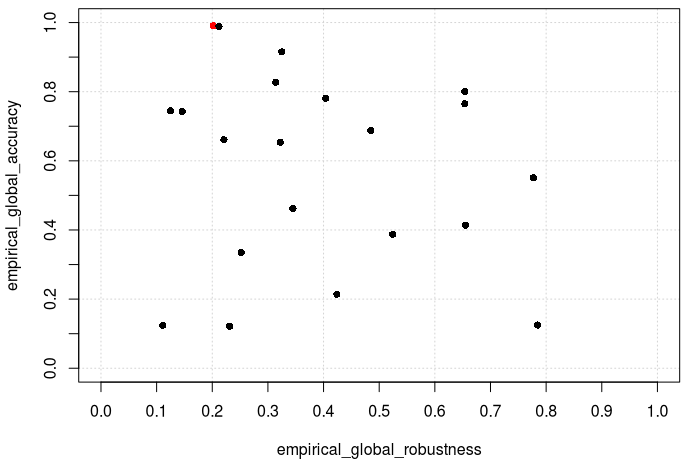
\includegraphics[scale=0.68]{my-graph-scatterplot.png}
	\captionsetup{labelformat=empty}
	\caption{Lo scatter plot di $\mathfrak{R}, \mathfrak{A}$ appena menzionato, su un totale di $20$ campioni di $\boldmath{s}$, bidimensionali uniformi}
\end{figure}

Osservando il grafico, appare che:

\begin{itemize}
	\item {Nessun modello prodotto presenta un'accuratezza peggiore o uguale a quella che si otterrebbe assegnando casualmente una classe a ciascun \textit{input} fornito;}

	\item {$3$ modelli prodotti presentano caratteristiche peggiori rispetto al classificatore di partenza, sia dal punto di vista della robustezza che dell'accuratezza;}

	\item {Nessun modello prodotto presenta un'accuratezza maggiore rispetto al classificatore fornito inizialmente;}

	\item {8 dei modelli prodotti presentano un'accuratezza inferiore allo $0.5$, comunemente considerato un limite di accettabilità del classificatore prodotto -- qualunque sia la sua robustezza;}

	\item {Per i modelli prodotti -- aventi accuratezza $>0.5$ e non peggiori del classificatore inizialmente fornito per entrambe le misure, è generalmente presente una correlazione negativa tra robustezza e accuratezza, anche se non è evidente una relazione \textit{monotòna} in tal senso.}

	\item {$2$ dei modelli prodotti, quelli aventi coordinate $(0.654, 0.765)$ e $(0.654, 0.801)$ presentano un profilo di accuratezza/robustezza confrontabile con quello di alcuni classificatori ottenibili tramite \textit{adversarial training} tradizionalmente inteso;}

\end{itemize}


Tali osservazioni, sebbene preliminari e rappresentative solamente di una singola possibile applicazione del modello proposto, costituiscono un risultato significativo. Considerate le molteplici difficoltà legate al -- noto tra l'altro -- problema di allenare un \textit{modello neurale generativo profondo}, esse non consentono di escludere come improduttiva la possibilità di indagare ulteriormente tale ambito d'applicazione, e anzi lasciano intuire la possibilità di produrre in tal senso classificatori in regimi di robustezza/accuratezza di potenziale interesse, anche se non necessariamente competitivi.


\begin{figure}[H]
	\centering
	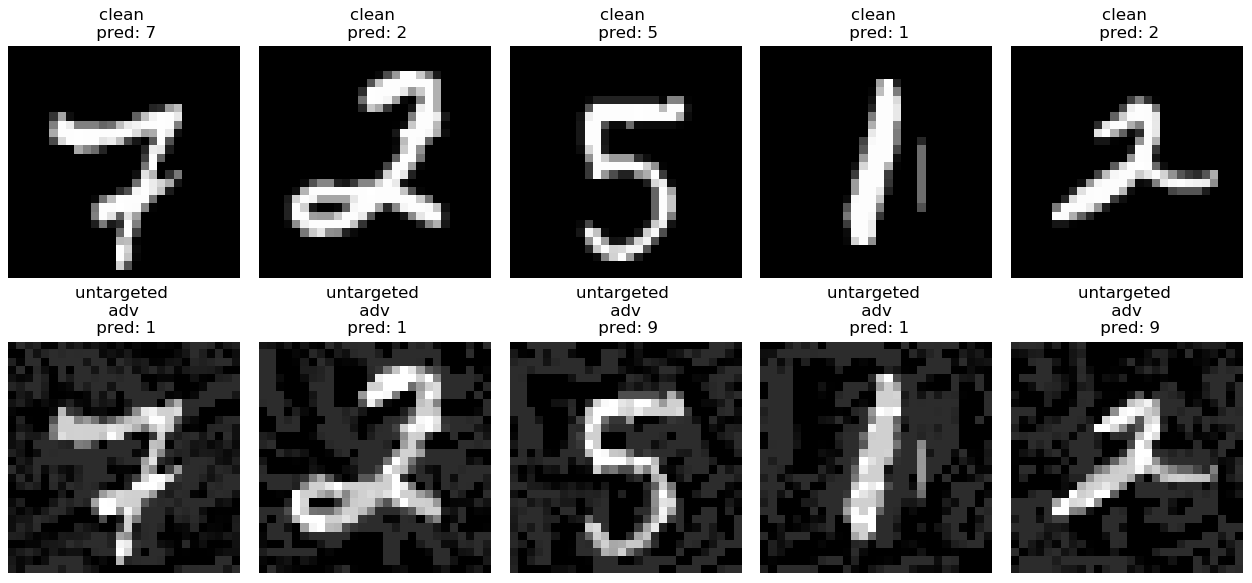
\includegraphics[scale=0.4]{mnist-adv-pgdlinf.png}
	\captionsetup{labelformat=empty}
	\caption{Un esempio di attacco PGD-Linf su $5$ esempi generati durante la procedura sperimentale seguita. Anche in tal caso, la vista umana è difficilmente ingannata -- come invece accade alla rete neurale utilizzata.}
\end{figure}


\newpage
\section{Conclusioni}

Nel corso del presente lavoro si è affrontata la tematica d'indagare se fosse possibile adottare soluzioni proprie del \textit{paradigma generativo} dell'apprendimento neurale profondo con lo scopo di produrre classificatori neurali -- anch'essi profondi e vulnerabili ad \textit{adversarial attacks} -- più robusti di quelli comunemente ottenuti tramite \textit{training} sulla base della sola accuratezza.

Pur dovendo confrontarsi con i tipici problemi relativi all'allenamento dei modelli generativi profondi fortemente sovraparametrizzati, è stato possibile osservare comportamenti d'interesse in relazione ad alcuni classificatori costruiti secondo tale modalità.

Nonostante quanto osservato non costituisca un'eccezione nel panorama delle metodologie aventi il medesimo scopo di quella proposta, il fatto che quest'ultima rappresenti un contributo originale al problema e sia stata studiata solamente in minima parte non può che essere ragione d'interesse verso tale nuova possibilità.

\subsection{\textit{Future work and suggestions}}

Direttamente collegata alla tematica d'indagine appena esposta è la possibilità di analizzare secondo termini più rigorosi le condizioni necessarie alla convergenza di un modello come quello proposto, e dei campioni estratti dal \textit{latent space} tali da determinare potenziali profili di accuratezza/robustezza d'interesse.

Di simile spirito, inoltre, potrebbe essere lo studio della topologia di suddetto \textit{latent space} -- in quanto basso-dimensionale e per questo approcciabile anche con tecniche di ottimizzazione multi-obiettivo, più tradizionali e sviluppate.

Sicuramente degna di ulteriore approfondimento è anche la questione di determinare se esiste -- e in tal caso di come sfruttare -- una misura differenziabile che possa essere associata all'accuratezza e alla robustezza di un classificatore neurale profondo, eliminando di conseguenza la necessità di utilizzo di un \textit{value network} per la stima di tale funzione.

Un'altra strada potenzialmente interessante, in parte già ritrovabile in Madry (2019) e Kurakin (2018), potrebbe essere percorsa andando ad utilizzare misure di robustezza dipendenti da norme diverse nel computo della \textit{empirical global robustness} di un modello.

Da ultimo -- e in maggior misura lontano dal tema specifico del lavoro presentato -- potrebbe essere degno d'indagine l'utilizzo, in fase di \textit{training}, di tecniche mutuate dall'ambito dell'apprendimento \textit{attivo} e \textit{continuo} per produrre una maggiore robustezza in un classificatore. O anche la determinazione di architetture neurali profonde in grado di esibire un comportamento robusto in maniera indipendente dai pesi, sulla strada in parte tracciata da Ha (2018).


% BIBLIOGRAPHY %
%------------------------------------------------------------------------%
\newpage
\nocite{*}
\bibliography{references}
\bibliographystyle{plain}
%------------------------------------------------------------------------%

\newpage
\appendix

\section{\textit{Small LeNet5}}

\subsection{Architettura (\textit{input-first})}
$\mathtt{Conv2D (channels in = 1, channels out = 8, kernel size = 5, stride = 1) }$\\
$\mathtt{MaxPool2D (kernel size = 2)}$\\
$\mathtt{ReLU}$\\
$\mathtt{Conv2D (channels in = 8, channels out = 16, kernel size = 5, stride = 1) }$\\
$\mathtt{MaxPool2D (kernel size = 2)}$\\
$\mathtt{ReLU}$\\
$\mathtt{Dropout (p = 0.25)}$\\
$\mathtt{Flatten (dimensions = 1)}$\\
$\mathtt{FC (channels in = 256, channels out = 64)}$\\
$\mathtt{ReLU}$\\
$\mathtt{Dropout (p = 0.5)}$\\
$\mathtt{FC (channels in = 64, channels out = 10)}$\\
$\mathtt{LogSoftmax (dimensions = 1)}$\\

\subsection{Parametri di training}
\begin{itemize}
	\item {Dataset split: \textit{train $90\%$}, \textit{test $10\%$}}
	\item {Training batch-size: $32$}
	\item {Epochs: $20$}
	\item {Loss: \textit{Categorical Cross-Entropy}}
	\item {Optimizer: \textit{Stochastic Gradient Descent with Momentum} ($\epsilon=0.01$, $\mu=0.5$)}
\end{itemize}

%%

\section{Generatore $\mathcal{G}$}

\subsection{Architettura (\textit{input-first})}
$\mathtt{UniformSample (dimensions = 2, interval = [-10,10]\times[-10,10])}$\\
$\mathtt{FC (channels in = 2, channels out = 32)}$\\
$\mathtt{LeakyReLU (slope = 0.07)}$\\
$\mathtt{FC (channels in = 32, channels out = 128)}$\\
$\mathtt{LeakyReLU (slope = 0.07)}$\\
$\mathtt{FC (channels in = 128, channels out = 512)}$\\
$\mathtt{LeakyReLU (slope = 0.07)}$\\
$\mathtt{FC (channels in = 512, channels out = 20522)}$\\
$\mathtt{Tanh}$\\

\subsection{Parametri di training}
\begin{itemize}
	\item {Optimizer: \textit{ADAM} ($\epsilon=0.01$,  $\beta_1=0.9$, $\beta_2=0.999$, \textit{decay} $=0.005$)}
\end{itemize}



%%


\section{\textit{Value network} $\mathcal{V}$}

\subsection{Architettura (\textit{input-first})}
$\mathtt{Flatten (dimensions = 1)}$\\
$\mathtt{FC (channels in = 20522, channels out = 512)}$\\
$\mathtt{LeakyReLU (slope = 0.02)}$\\
$\mathtt{FC (channels in = 512, channels out = 32)}$\\
$\mathtt{LeakyReLU (slope = 0.02)}$\\
$\mathtt{FC (channels in = 32, channels out = 2)}$\\
$\mathtt{Sigmoid}$\\

\subsection{Parametri di training}
\begin{itemize}
	\item {Optimizer: \textit{ADAM} ($\epsilon=0.35$,  $\beta_1=0.9$, $\beta_2=0.999$, \textit{decay} $=0.015$)}
	\item {Calcolo di $\mathfrak{R}, \mathfrak{A}$ sull'intero dataset (\textit{elements=$10000$})}
\end{itemize}




\newpage

\section*{Ringraziamenti}

In conclusione del presente lavoro desidero ringraziare i miei genitori, per la loro insostituibile vicinanza, per il sostegno e la forte compartecipazione a gioie e difficolta di questo percorso, e per avermi trasmesso la curiosità verso ciò che è nuovo e incompreso. E mio nonno -- che ricordo spesso con affetto -- per avermi mostrato con l'esempio la tenacia.

Molto devo al mio relatore, il prof. Bortolussi, per il supporto fino all'ultimo istante, l'inesauribile pazienza, la sempre viva attenzione verso ambiti di ricerca in costante cambiamento. Spero di aver assorbito da lui anche solo un pizzico del suo atteggiamento verso l'entusiasmante mondo dell'\textit{Intelligenza Artificiale}, un atteggiamento aperto, interessato alla costruzione di fondamenta robuste e libero da \textit{overfitting} sulle mode del momento.

Un ringraziamento va al mio co-relatore, il prof. Benatti, in special modo per la grande disponibilità e comprensione -- anche in un periodo d'emergenza come quello attuale.\\
E al prof. Pastore per essere sempre stato un saldo punto di riferimento.

Grazie anche a Francesco Cicala, per le lunghe conversazioni -- accademiche e non -- e per l'instancabile capacità di farmi vedere le cose da una prospettiva sempre diversa e mai scontata.

Infine, grazie ai professori, ricercatori e studenti parte del \textit{Bortolussi Group} per l'amichevole accoglienza e per i ricchi e brillanti spunti che quotidianamente mi hanno offerto e continuano ad offrire.

\end{document}
